\listfiles
\documentclass[a4paper]{article}
\usepackage[T2A]{fontenc}
\usepackage[english,russian]{babel}
\usepackage{sectsty}
\sectionfont{\centering\normalfont}
\subsectionfont{\centering\normalfont}
\subsubsectionfont{\normalfont}
\usepackage{changepage}
\usepackage{filecontents}
% \usepackage{mathptmx}
\usepackage{float} 
\usepackage{subcaption}
\usepackage[utf8]{inputenc}
\usepackage[14pt]{extsizes}
\usepackage{physics} 
\usepackage{graphicx}
\graphicspath{{../misc/}}
\usepackage{setspace,amsmath}
% \usepackage[left=30mm, right=15mm, top=20mm, bottom=20mm]{geometry} 
\usepackage[nottoc]{tocbibind}
\usepackage[style=gost-numeric,sorting=none,backend=biber,defernumbers=false]{biblatex}
\DeclareBibliographyAlias{misc}{article}
\addbibresource{lit.bib} 
%%%%%%%%%%%%%%%%%%%%%%%%%%%%%%%%%%%%%
% \everymath{\displaystyle}
\DeclareMathSizes{12}{20}{14}{10}

\makeatletter
\def\@makefnmark{\hbox{\@textsuperscript{\normalfont(\@thefnmark)}}}
\makeatother
 
\captionsetup[figure]{labelsep=period}
\captionsetup[table]{labelsep=period}

\usepackage{titling,lipsum}

\usepackage{hyperref}
\hypersetup{
    colorlinks,
    citecolor=black,
    filecolor=black,
    linkcolor=black,
    urlcolor=blue
}

\begin{document}

\thispagestyle{empty}

\begin{center}
    \large\textbf{Обучение связей конкуренции локальных рецептивных полей в спайковых нейронных сетях}\\
    \hfill\break
    
    Даниил Гафни, Дмитрий Нехаев, Вячеслав Дёмин
\end{center}


\tableofcontents


\pagebreak

\addcontentsline{toc}{section}{Аннотация}
\section*{Аннотация}
Стандартные методы обучения весов связей, применяющиеся в формальных нейронных сетях (метод обратного распространения ошибки) затруднительно применять к спайковым нейронным сетям из-за их дискретной и распределенной во времени природы. Хотя такие проекты существуют, больший интерес представляют локальные алгоритмы обучения, являющиеся более биологически корректными, способными обеспечить самообучение алгоритма (без учителя) и более энергоэффективными (при условии реализации на специализированном аппаратном оборудовании). 

Одним из основных недостатков СНС по сравнению с формальными НС является слабая изученность локальных правил обучения, и ввиду этого, более низкие показатели точности работы (логического вывода) алгоритмов на основе СНС. Таким образом, исследование алгоритмов обучения СНС, таких как STDP, является важной задачей. 

Введение связей конкуренции (имеющих отрицательные веса) позволяет добиться лучшего разделения выучиваемых нейронами признаков. Обучение этих связей, возможно, позволит добиться еще более хороших результатов за счет организации кооперативной или конкурентной работы групп нейронов.

% \cite{Lee_2020, backprop_spiking}

\pagebreak

\addcontentsline{toc}{section}{Введение}
\section*{Введение}
Спайковые нейронные сети являются перспективным нейроморфным алгоритмом, биологически корректно моделируя взаимодействия нейронов мозга. Наибольший интерес СНС представляют для решения задач в реальном времени (принятие решений, распознавание образов), так как могут быть реализованы на специализированном вычислительно- и энергоэффективном нейрочипе (например, на основе мемристоров).

Современные формальные нейронные сети отлично справляются со многими задачами машинного обучения \cite{pmlr-v28-wan13, Khan_2020}. Однако их обучение --- трудоемкий процесс, требующий больших вычислительных ресурсов. Обычно обучение ведется на десятках и сотнях тысяч примеров и может занимать месяцы. Как само обучение, так и последующее применение формальных нейросетевых алгоритмов далеки от эффективности \cite{Edwards2015GrowingPF}. Это связано как с физически раздельным хранением значений весов и активаций нейронов, так и с самими вычислениями, которые носят тензорный характер --- связанный с векторно-матричным и матрично-матричным умножением чисел с плавающей запятой. Современные процессоры не оптимизированы для подобных вычислений. Гораздо лучше традиционных процессоров для этих задач подходят GPU --- архитектуры, изначально созданные для работы с компьютерной графикой, а потому более подходящие для тензорных вычислений, однако и они не дают желаемого результата. Число параметров в современных формальных нейронных сетях может достигать сотен миллионов \cite{ManyParams, Khan_2020}.

Спайковые нейронные сети имеют ряд преимуществ перед формальными нейронными сетями.

\begin{itemize}
\item С помощью спайковых нейронных сетей возможно более богатое динамичное кодирование паттернов в непрерывном времени, которое, как правило, недоступно для формальных нейронных сетей \cite{Ismail_Fawaz_2019}.
\item Для обучения спайковых нейронных сетей могут применять локальные алгоритмы \cite{STDP, pehlevan2019spiking, Baldi_2016}, которые используют для обновления веса каждой связи лишь информацию от соединяемой данной связью нейронов. Напротив, при обучении формальных нейронных сетей для обновления веса каждой связи используется информация о всех нейронных связях, стоящих между этой связью и выходом сети. Таким образом, сами по себе алгоритмы обучения спайковых нейронных сетей являются более эффективными, чем алгоритмы обучения формальных нейронных сетей.
\item Более того, эти алгоритмы могут использовать обучение без учителя (unsupervised learning), для которого не требуется ручной разметки данных, как в случае использования методов обратного распространения ошибки.
\item Спайковые нейронные сети могут быть реализованы на специализированном сверхэнергоэффективном (достигается за счет сокращения количества актов и средней длины передачи сигналов, а также пространственной и временной разреженности спайков в сети) нейроморфном процессоре. Такая реализация вместе с чисто алгоритмическим преимуществом спайковых нейронных сетей дает также существенный выигрыш в производительности. \cite{hardware1, hardware2}. 
\item Спайковые нейронные сети в большей степени, чем формальные нейронные сети, биологически корректно моделируют взаимодействия нейронов, что может использоваться для биологических симуляций нервной системы в целях не только биоинформатических, но также биофизических и медицинских аспектов функционирования.
\end{itemize}

Представляет интерес изучение известных архитектур спайковых нейронных сетей и их топологий, в том числе классических архитектур формальных нейронных сетей --- сверточной, локально соединенной и полносвязной \cite{Khan_2020}. Более того, введение дополнительных рекуррентных связей конкуренции в этих архитектурах способствует лучшему разделению признаков в  процессе обучения \cite{MaxActiv1, MaxActiv2}. Полносвязная сеть --- максимально простая модель, которая может использоваться в качестве сравнительного эталона. Сверточная и локально соединенная архитектуры используют свертку --- операцию, позволяющую более эффективно (по сравнению с полносвязной сетью) выделять важные признаки. Локально соединенная архитектура особенно интересна тем, что легко реализуется аппаратно, так как, в отличие от сверточной сети, не использует общих синаптических весов. Локально соединенная архитектура имеет значительно меньшее количество параметров, чем полносвязная и в то же время позволяeт обучать уникальный набор признаков для каждого рецептивного поля, в отличие от сверточных сетей. В то же время, сверточные сети обладают трансляционной инвариантностью --- полезным свойством для обработки изображений. Наличие конкуренции в нейронных сетях позволяeт делать их признаки более независимыми. Поэтому для экспериментов были выбраны локально соединенные и сверточные сети со связями конкуренции, а в качестве базовой модели --- полносвязная сеть со связями конкуренции.

\clearpage

На сегодняшний день разрабатывается несколько десятков нейроморфных процессоров для аппаратной реализации спайковых нейронных сетей. К одним из них относятся: TrueNorth, разработанный IBM (2014), созданная совместными усилиями Netflix и Google платформа SpiNNaker (2015), проект Intel --- Loihi (2017) и Akida --- нейроморфный процессор от BranChip (2020). В таблице \ref{hardware_snn} проведено сравнение данных аппаратных нейроморфных решений по ключевым параметрам, а также указаны аналогичные параметры человеческого мозга.

\begin{table}[h]
 \caption {Сравнительная таблица аппаратных реализаций спайковых нейронных сетей. Указано энергопотребление при решении типичной задачи машинного обучения.}
 \begin{center}
  \begin{tabular}{|c|c|c|c|}
  \hline
  {Название} & {Нейроны} & {Синапсы} & {Энергопотребление, мВт}\\
  \hline
  {Мозг человека \cite{human_brain}} & {$\approx 16 \cdot 10^9$} & {$\approx 1 \cdot 10^{14}$} & {20000}\\
  \hline
  {TrueNorth \cite{TrueNorth}} & {$1 \cdot 10^6$} & {$256 \cdot 10^6$} & {64\footnotemark[1]}\\
  \hline
  {SpiNNaker \cite{SpiNNaker}} & {$1 \cdot 10^9$} & {$1 \cdot 10^{12}$} & {1000\footnotemark[2]}\\
  \hline
  {Loihi \cite{Loihi}} & {$130 \cdot 10^3$} & {$130 \cdot 10^{6}$} & {неизвестно}\\
  \hline
  {Akida \cite{Akida}} & {$1.2 \cdot 10^6$} & {$10 \cdot 10^{9}$} & {$\sim 10$ \footnotemark[3]}\\
  \hline 
  \end{tabular}
 \end{center}
\label{hardware_snn}
\end{table}

\footnotetext[1]{Для обработки видео разрешением $400 \times 240$ пикселей 30 кадров/с.}
\footnotetext[2]{При полной загрузке.}
\footnotetext[3]{Энергопотребление может быть от 1 мкВт до 10 мВт в зависимости от сложности задачи.}

Все эти проекты разрабатываются под современные нужды и уже способны применяться в исследованиях или индустрии, что еще раз подчеркивает важность исследования спайковых нейронных сетей.

В настоящей работе:
\begin{enumerate} 
\item Изучается влияние обучения связей конкуренции \cite{MaxActiv1, MaxActiv2, hardware_survey} между нейронами на точность распознавания образов в задаче классификации рукописных изображений цифр из датасета MNIST \cite{MNIST} при обучении без учителя для архитектуры локально соединенной сети (Locally Connected Spiking Neural Network, LCSNN) \cite{saunders2019locally}.

\item Проводится сравнение этой архитектуры со сверточной сетью (Convolution Spiking Neural Network, CSNN) и полносвязной сетью (Fully Connected Spiking Neural Network, FCSNN).

\end{enumerate}

\clearpage

\section{Обучение спайковой нейронной сети с необучаемой конкуренцией локальных рецептивных полей}

\subsection{Описание задачи}
Для работы была выбрана классическая задача машинного обучения --- задача классификации изображений рукописных цифр из набора данных MNIST. MNIST состоит из размеченных обучающей и тестовых выборок объемами 60000 и 10000 изображений. Изображения имеют размер 28 $\times$ 28 пикселя и являются черно-белыми. Из-за необходимости калибровки сетей (\ref{calibration}) обучающая выборка была разбита на 50000 изображений для обучения (обучающая выборка) и 10000 изображений для калибровки (калибровочная выборка).
 

% \begin{figure}[H] \label{MNIST} 
% \begin{center}
%  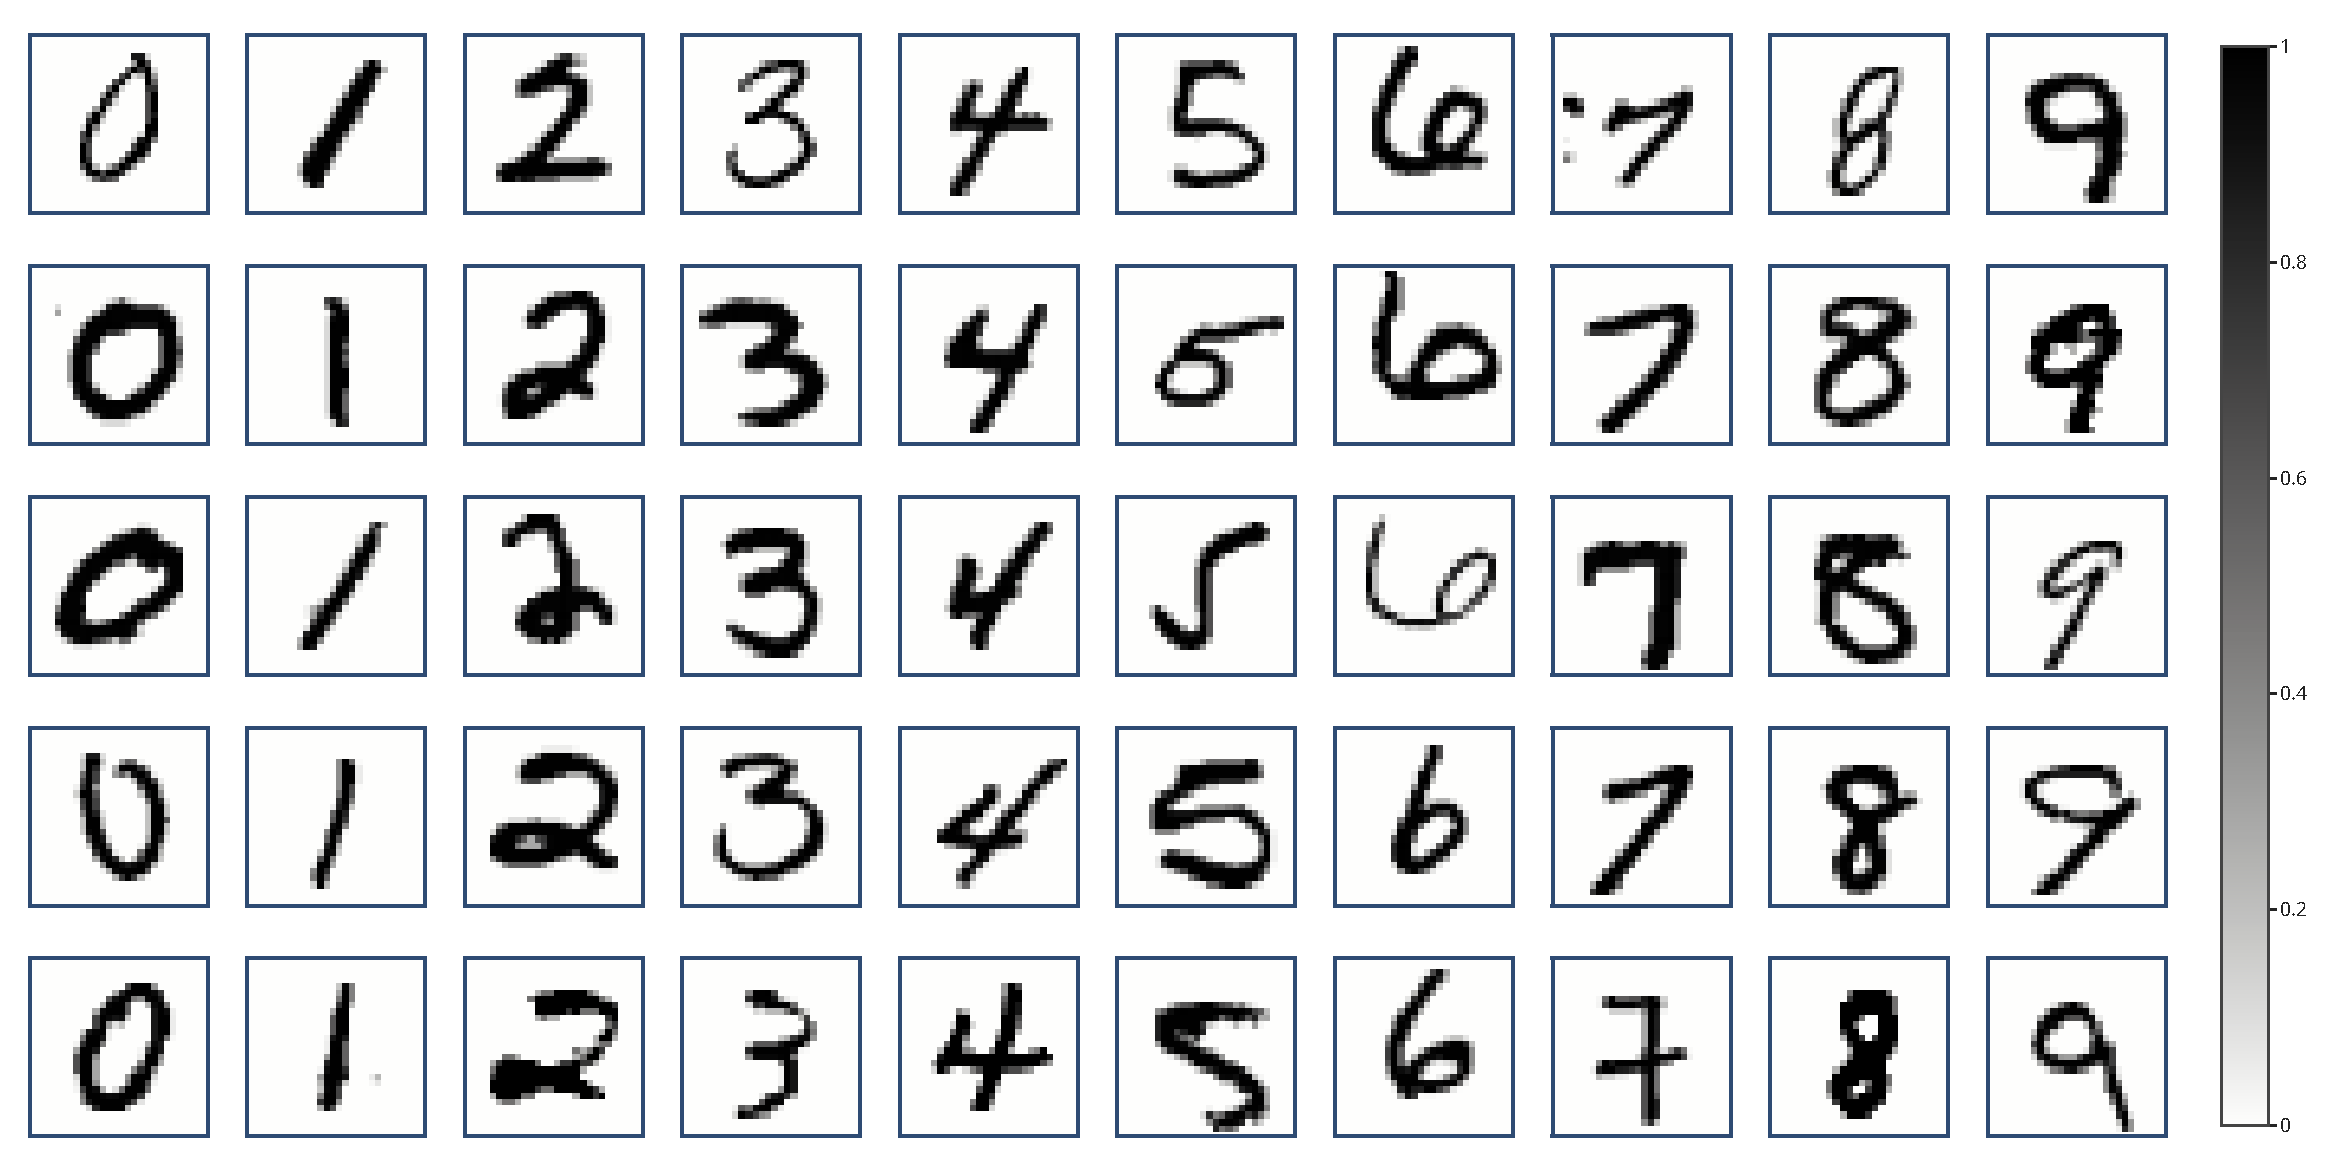
\includegraphics[,
%  width=\textwidth,keepaspectratio=true]{MNIST.pdf} 
%  
%  \caption{Изображения MNIST}
% \end{center}
% \end{figure}


В этой работе изображения обрезаются так, что используется только центральная область 20$\times$20 пикселей.\\

\subsection{Особенности архитектуры сетей с конкуренцией}
В данной работе изучаются сети с использованием локально соединенных, полносвязных и сверточных слоев.

\begin{itemize}
 \item \textbf{Полносвязный слой} - в нем каждый нейрон соединен с каждым нейроном из предыдущего слоя.
 \item \textbf{Сверточный слой} - в нем нейроны разделены на каналы. Веса всех нейронов в одном канале совпадают. Каналы равноправны, а каждый нейрон в канале соединен только с некоторой областью (прямоугольной в случае двумерного слоя) \cite{li2020survey}.
 \item \textbf{Локально соединенный слой} - он совпадает со сверточным слоем, но каждый нейрон имеет свои уникальные веса \cite{saunders2019locally}.
\end{itemize}

Топология сетей с конкуренцией включает в себя равноправные (расположенные в одном слое и имеющие аналогичные связи) нейроны, соединенные друг с другом синоптическими связями с отрицательным весом. Так как общий вид этих сетей совпадает, рассмотрим его на примере сети с локально соединенным слоем.

Нейросетевая архитектура LCSNN вдохновлена строением зрительной коры мозга. $Y$ слой сети состоит из $n$ каналов, каждый из которых является локально соединенным с $X$ слоем нейронов.

\begin{figure}[H] \label{LCSNN}
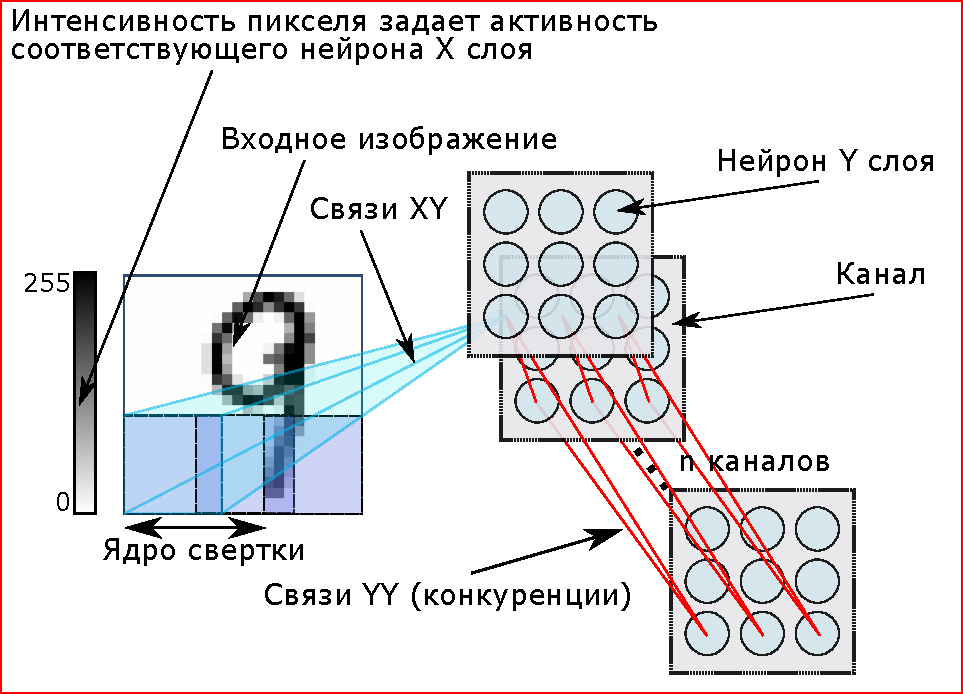
\includegraphics[,
 width=\textwidth,keepaspectratio=true]{LCSNN_ru.pdf} 
    \caption{Схема архитектуры LCSNN} 
\end{figure}

Нейроны, имеющие общие рецептивные поля, соединяются $YY$ связями конкуренции. Такие связи имеют отрицательные веса, а значит, негативно влияют на активность. Нейроны, не имеющие общего рецептивного поля (а значит, реагирующие на разные области изображения) не конкурируют между собой. Связи конкуренции вводятся для улучшения разделения нейронов по выучиваемым признакам. Аналогичная архитектура может быть построена для сетей с использованием сверточных или полносвязных слоев.

В этой работе используется Adaptive Integrate-And-Fire (ALIF) модель нейронов. Динамика потенциала нейрона в этой модели задается уравнением

\begin{equation} \label{eq:alif}
 \tau_v \dv{v(t)}{t} = -v(t) + v_{rest} + I(t) \cdot R \text{,}
\end{equation} где $I(t)$ --- ток, накопившийся в нейроне к моменту времени $t$, $v_{rest}$ --- уровень релаксации, $\tau_v$ --- временная константа симуляции, а $R$ --- размерный коэффициент, численно равный 1.\\ 

Таким образом, потенциал нейрона сам по себе стремится вернуться в состояние релаксации, так как если $I(t) = 0$ (нет входящих спайков) и $v(t) = v_{rest}$, то производная $\dv{v(t)}{t} = 0$, то есть потенциал нейрона будет оставаться постоянным на уровне $v_{rest}$. 

Порог активации $v_{thresh}$ у ALIF нейрона не является константой, а немного повышается при каждом спайке, релаксируя затем к своему начальному значению $\theta_o$. Динамика порога активации задается следующими уравнениями:
\begin{equation} 
 v_{thresh} = \theta_0 + \theta(t) \text{,}
\end{equation} где $\theta_0$ --- начальный порог активации, $\theta(t)$ --- адаптивная добавка, которая вычисляется из условия\\

\begin{equation}
 \tau_v \dv{\theta(t)}{t} = -\theta(t)
\end{equation}\\

Также после испускания каждого спайка адаптивная добавка $\theta(t)$ повышается на $\theta_{plus}$.

Таким образом, порог активации нейрона сам по себе стремится вернуться к начальному значению, так как при $\theta(t) = \theta_0$, то производная $\dv{\theta(t)}{t} = 0$, то есть порог активации нейрона будет оставаться постоянным на уровне $\theta_0$.\\

После испускания каждого спайка наступает короткий период рефрактерности, при котором на протяжении времени $t_{refract}$ потенциал нейрона остается на уровне $v_{reset}$.

% \begin{center}
% \begin{figure}[H]
%  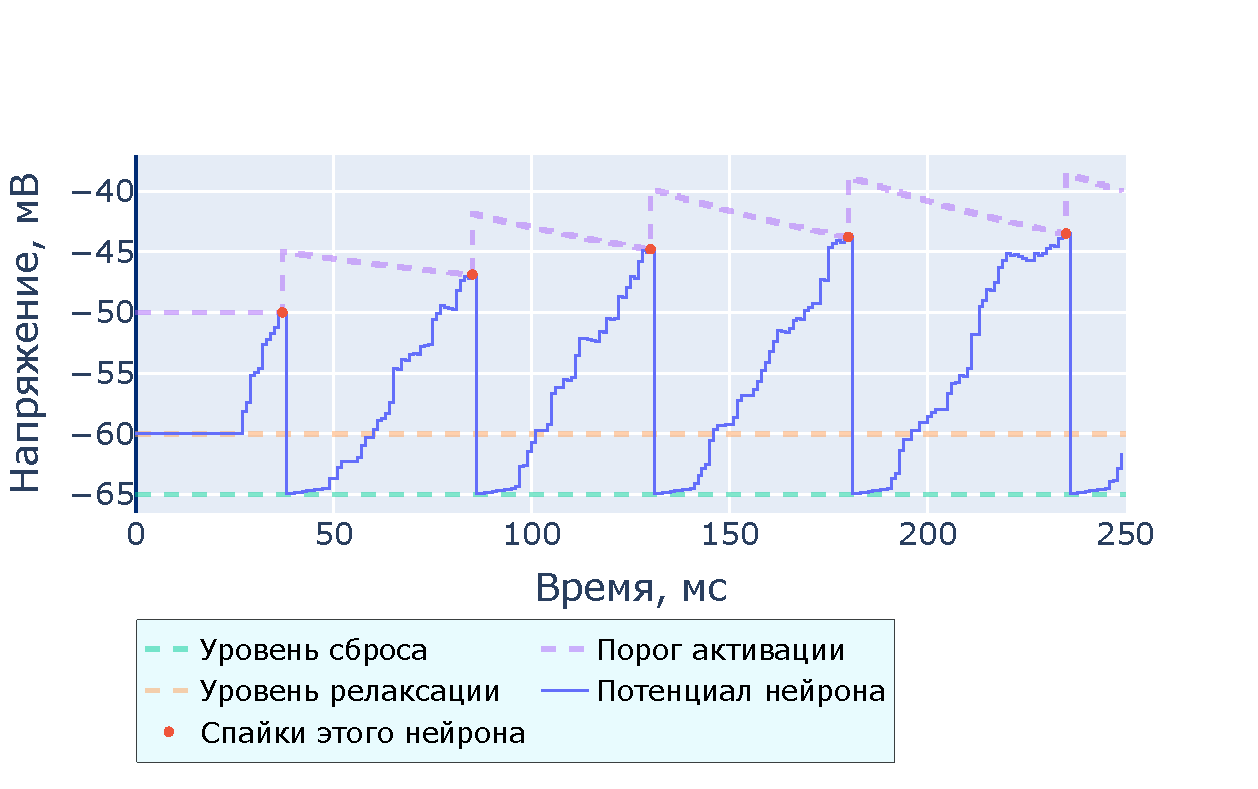
\includegraphics[width=\textwidth,keepaspectratio=true]{model_alif_ru.pdf}
%  \caption{Типичная зависимость потенциала порогового интегратора с утечкой и адаптивным порогом от времени. Красными точками отмечены спайки нейрона. Видны скачки порога активации после испускания спайков и его постепенное возвращение к исходному уровню.\\
%  \textit{Примечание: здесь исключительно для наглядности используется такое большое значение $\theta_{plus}$, в реальных экспериментах его влияние менее значительно.}}
% \end{figure} 
% \end{center}

Начальные веса связей задаются случайными числами из равномерного распределения.

\subsection{Обучение прямых связей}
Для уменьшения числа параметров модели изображения обрезаются до размера 20$\times$20 пикселей. Края изображений часто практически пусты, поэтому эта операция практически не влияет на объем информации, доступный сети. Для каждого изображения при помощи распределения Пуассона с математическим ожиданием, пропорциональным интенсивности соответствующего пикселя, генерируются $X$ спайки. Обучение связей $XY$ производится по правилу STDP \cite{STDP}. Это биологически инспирированное правило обучения без учителя \cite{STDP}. При получении пре-спайка и испускании пост-спайка вес $w$ связи, по которой пришел пре-спайк, увеличивается на $\Delta w$, где
\begin{equation} 
\Delta w =
 \begin{cases}
 A_+ \cdot e^{- \frac{t_{pre} - t_{post}}{\tau_+}}, t_{pre} - t_{post} > 0\\
 A_- \cdot e^{- \frac{t_{pre} - t_{post}}{\tau_-}}, t_{pre} - t_{post} < 0
 \end{cases}
\end{equation}

Заметим, что

$$
\begin{cases}
 A_{+} > 0\\
 A_{-} < 0
\end{cases}
$$

% \begin{figure}[H] \label{fig:STDP} 
% \begin{center}
%  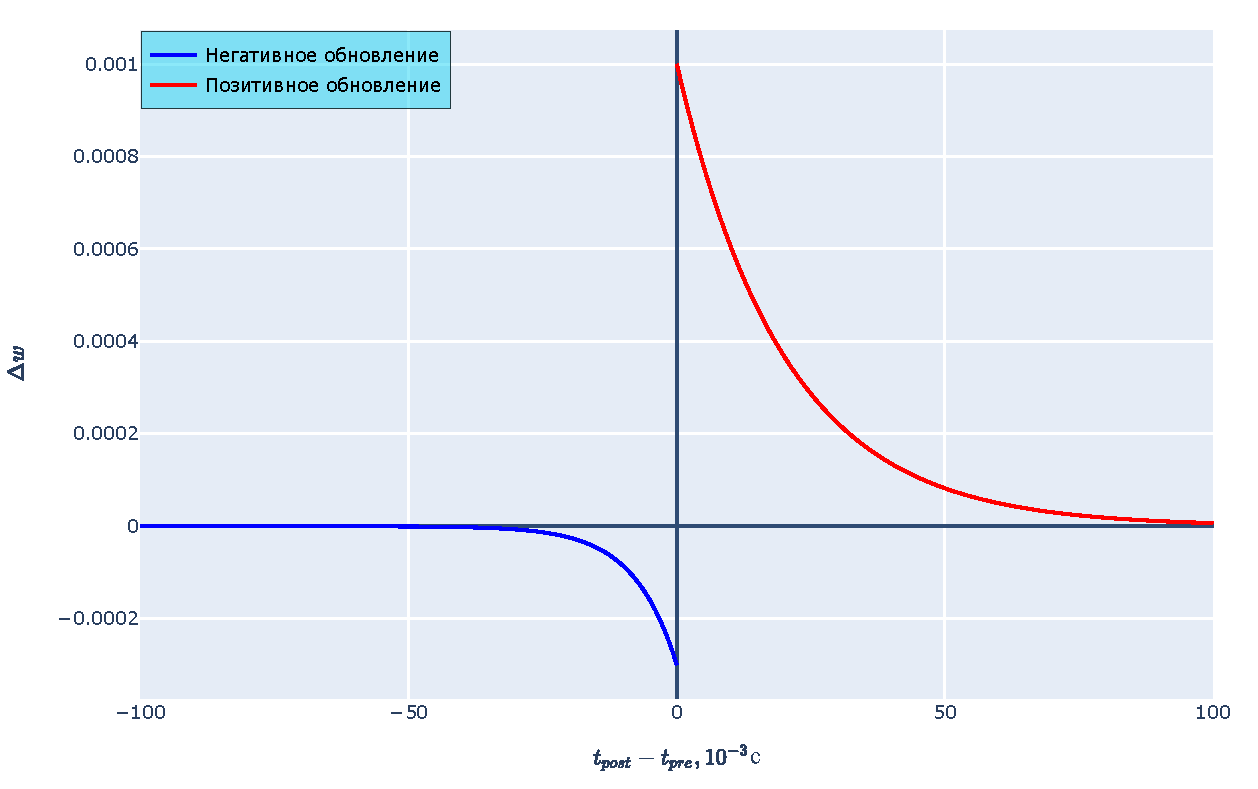
\includegraphics[,
%  width=\textwidth,keepaspectratio=true]{STDP_ru.pdf}
%  
%  \caption{Правило STDP. График зависимости изменения веса от разности времени регистрации пост- и пре- спайков.}
% \end{center}
% \end{figure}

Таким образом, в процессе обучения у каждого нейрона увеличивается вес связей, по которым систематически пре-спайк приходит перед излучением пост-спайка, и наоборот, вес уменьшается у тех связей, для которых такой закономерности не наблюдается. После такого обучения нейрон начинает активнее реагировать на пре-спайки от нейронов, соединенных с ним связями с большими весами, а значит, начинает сам испускать пост-спайк, если в короткий промежуток времени эти нейроны будут активны одновременно. Этим он объединяет их активность, посылая пост-спайк дальше по сети. Обратное правило (с отрицательными $A_{+}$ и $A_{-}$), называется правилом anti-STDP. В настоящей работе оно используется для обучения связей конкуренции.

После каждой итерации обучения производится нормализация весов --- веса каждого нейрона умножаются на такое число, чтобы их сумма стала равной определенной константе. Это делается для избежания возникновения слишком больших отдельных весов. Значение константы нормализации есть важный гиперпараметр модели, который подбирается для каждой конкретной архитектуры.

\begin{figure}[H]
\centering
\begin{subfigure}{0.45\textwidth}
    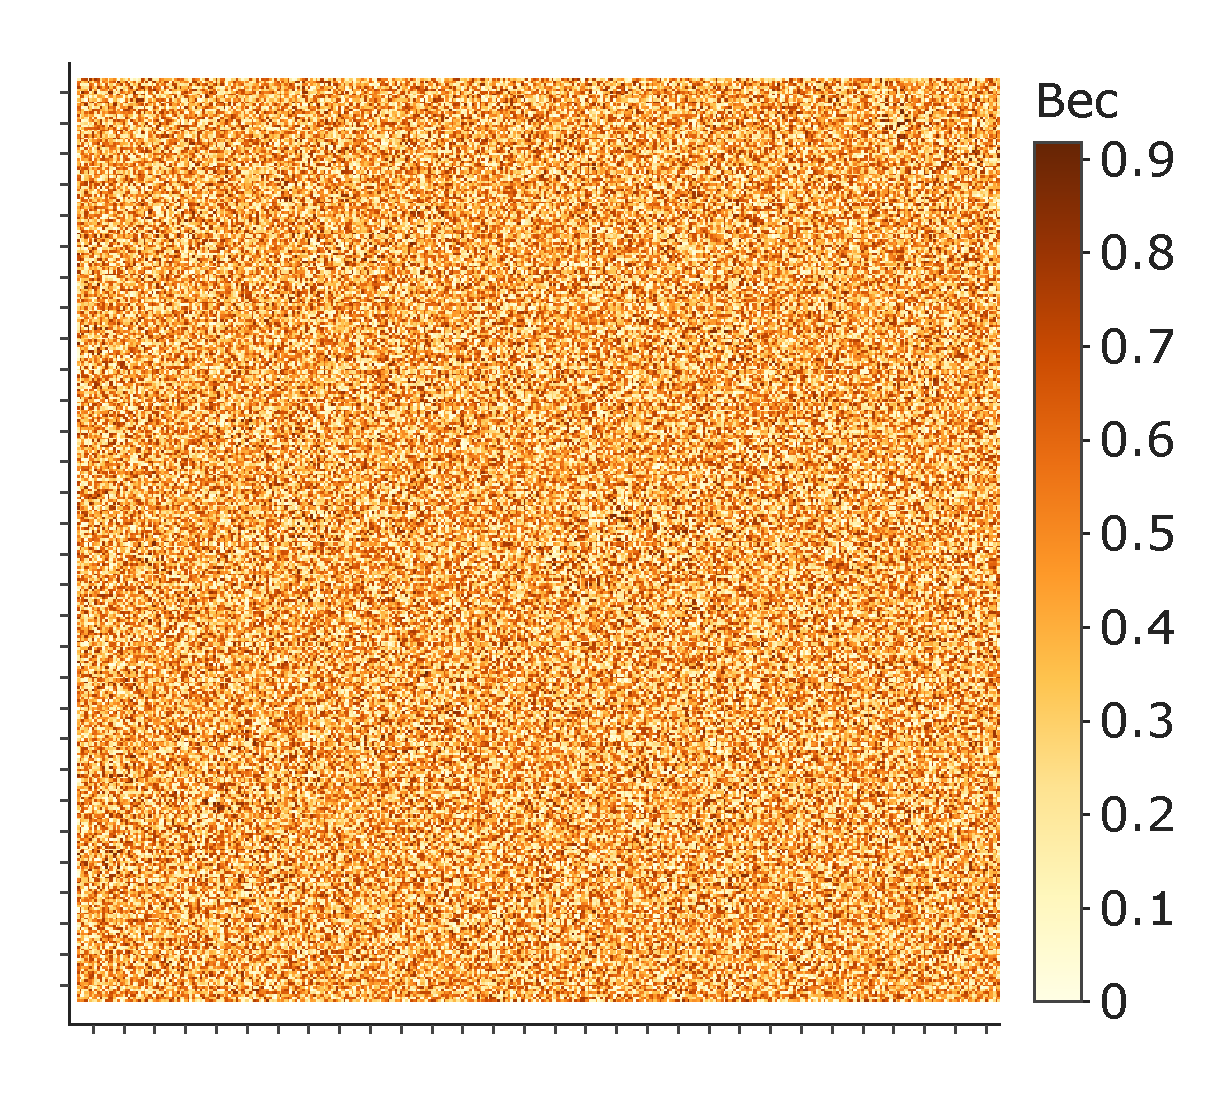
\includegraphics[width=\textwidth,keepaspectratio=true]{weights_XY_untrained_ru.pdf}
    \caption{Перед обучением}
\end{subfigure}
\begin{subfigure}{0.45\textwidth}  \label{weights_XY}
    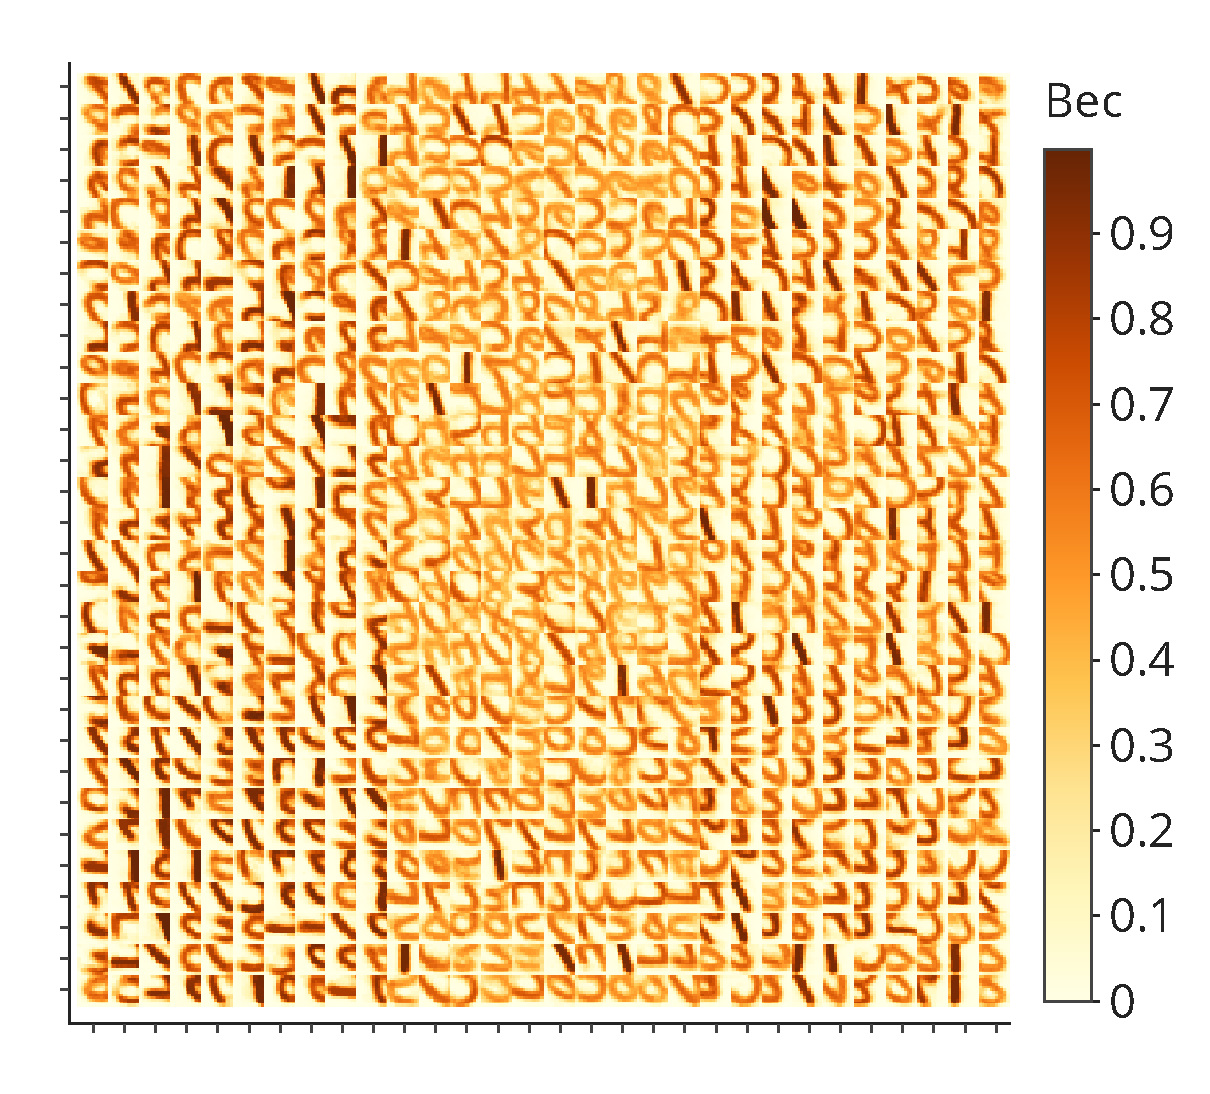
\includegraphics[width=\textwidth,keepaspectratio=true]{weights_XY_ru.pdf}
    \caption{После 10000 итераций обучения}
\end{subfigure} 
\caption{Визуализация весов $XY$ связей. Каждый квадратик 12$\times$12 соответствует весам одного $Y$ нейрона. Видно, что после обучения нейроны выучивают некоторые признаки, в которых явно угадываются элементы цифр.}
\end{figure}

\subsection{Интерпретация активности спайковой нейронной сети}

Для интерпретации активности нейронов $Y$ слоя сети использовалось несколько методов.

\begin{itemize}
 \item Голосование патчей
 \item Общее голосование нейронов
 \item Голосование нейронов с предварительным отбором по спайкам
 \item Линейный классификатор
\end{itemize}

Преимущество первых трех методов заключается в их простоте. Однако, линейный классификатор значительно превосходит их по точности.\\

\subsubsection{Калибровка голосов} \label{calibration}
Для первых трех методов необходимо произвести калибровку голосов нейронов. Каждому нейрону $Y$ слоя ставится в соответствие 10 чисел (голосов) для каждого возможного класса цифр (от 0 до 9). Голос вычисляется как усредненное по различным изображениям число спайков данного нейрона в ответ на демонстрацию сети данной цифры (на протяжении всего времени симуляции) ---
$$vote = \frac{\sum_{1}^{n} {\sum_{0}^{t_{max}} s_t}}{n} \text{, где}$$
$s_t$ принимает значение 0 или 1 в зависимости от наличия спайка в данный момент времени, $n$ --- размер калибровочной выборки.

Для всех сетей использовалась калибровка на 10000 примерах из калибровочной выборки. Заметим, что калибровка не является частью обучения сети, так как она входит лишь в алгоритм интерпретации поведения сети. Эти голоса используются как мера уверенности нейрона в каждом из классов. После демонстрации изображения сети подсчитывается общее количество спайков для каждого нейрона $Y$ слоя.

\begin{figure}[H]
\centering
\begin{subfigure}{\textwidth}
    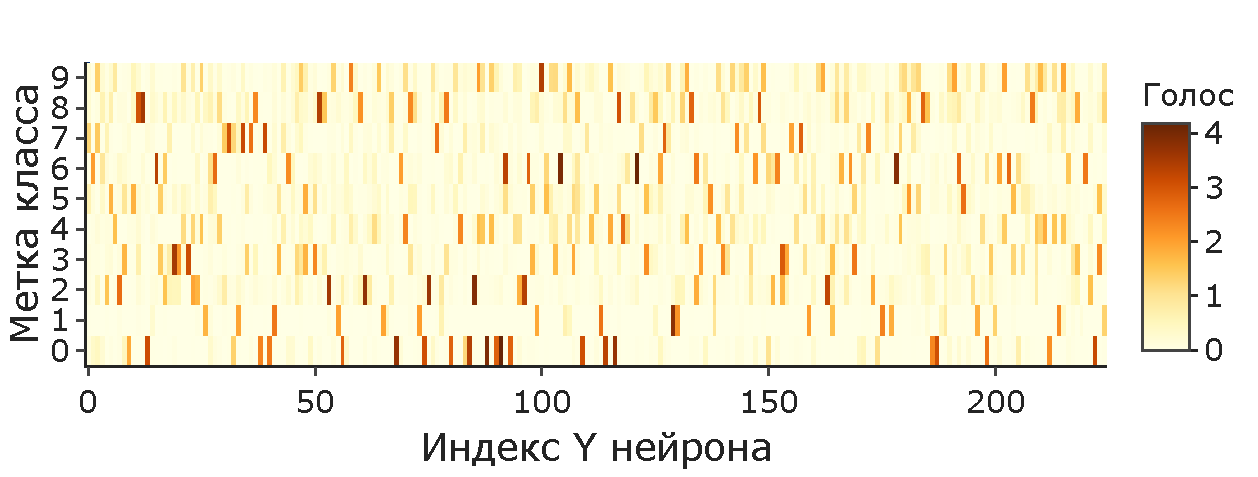
\includegraphics[width=\textwidth,keepaspectratio=true]{votes_ru.pdf}
    \caption{Голоса нейронов.}
\end{subfigure}
\begin{subfigure}{\textwidth} 
    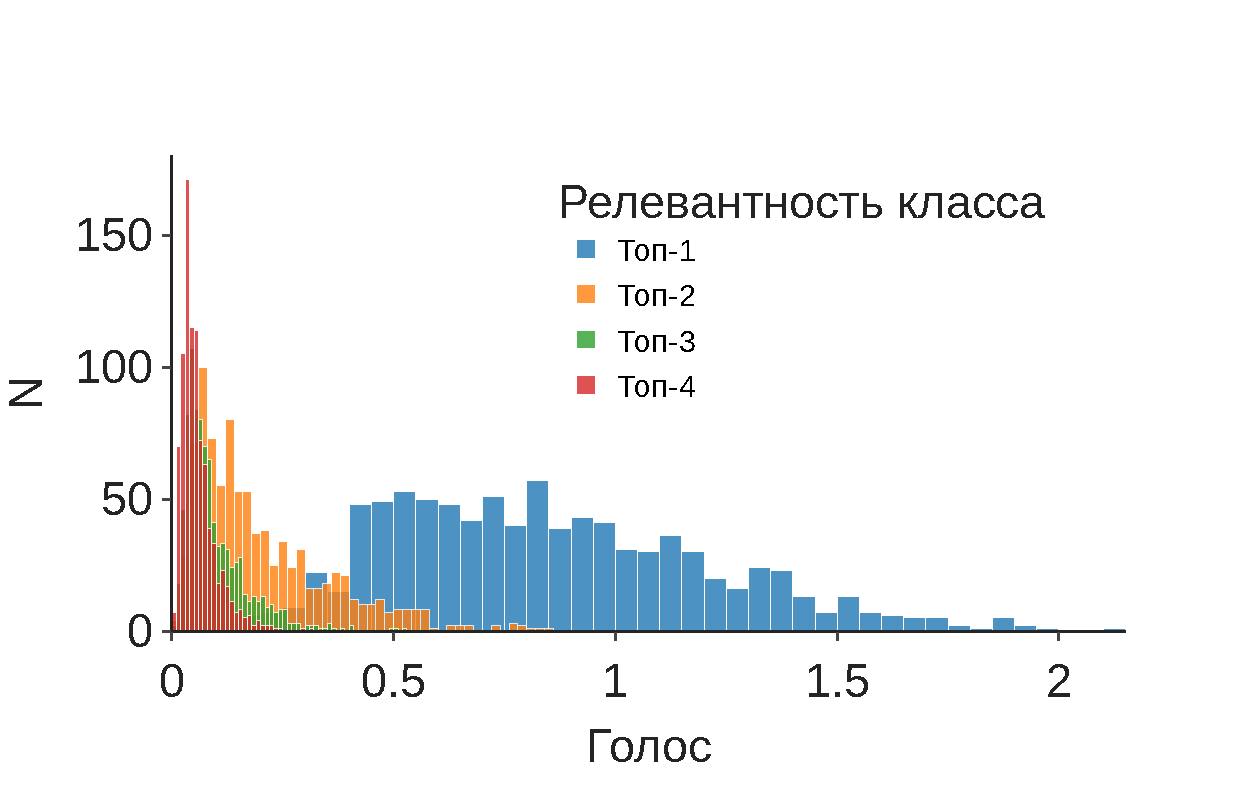
\includegraphics[width=\textwidth,keepaspectratio=true]{votes_distr_4_ru.pdf}
    \caption{Распределения голосов нейронов по четырем наиболее релевантным классам (для каждого нейрона). Видно, что величина голоса сильно падает с уменьшением релевантности.}
\end{subfigure}
\caption{Визуализация голосов нейронов $Y$ слоя. Высокие значения соответствуют большой специализации нейрона на соответствующем классе.}
\end{figure}

Далее результатом будем называть произведение количества спайков нейрона на голос.

\begin{center}
 Общее голосование
\end{center}
Ответом сети считается класс с максимальным результатом среди всех нейронов.

\begin{center}
 Голосование патчей
\end{center}
Для каждого рецептивного поля ищется нейрон с максимальным результатом. Ответом сети считается класс с максимальным результатом среди таких нейронов для всех рецептивных полей.

\begin{center}
 Отбор по спайкам
\end{center}
Для каждого рецептивного поля ищется нейрон с максимальным количеством спайков. Ответом сети считается класс с максимальным результатом среди таких нейронов для всех рецептивных полей.

\begin{center}
 Линейный классификатор
\end{center}
Суммы спайков отдельных нейронов $Y$ слоя используются для обучения с учителем линейного классификатора. Для обучения классификатора также используется калибровочная выборка.

\begin{center}
 Оценка алгоритма интерпретации активности
\end{center}
Для оценки работы алгоритма интерпретации используется точность --- отношение количества верно распознанных цифр к размеру тестовой выборки. В этой работе во всех случаях размер тестовой выборки составляет 10000. 

\subsubsection{Сравнение алгоритмов интерпретации активности сети}
Были построены кривые обучения для различных алгоритмов интерпретации активности сети. Точность измерялась через каждые 250 итераций обучения. Для калибровки алгоритма интерпретации использовалась калибровочная выборка объемом 5000. Для измерения точности использовалась тестовая выборка объемом 1000.

Видно, что через несколько тысяч итераций обучения точность распознавания выходит на плато насыщения, после чего уже не возрастает. Видно, что три метода голосования в целом не отличаются по точности, а линейный классификатор значительно превосходит их все. Заметим, что точность даже необученной сети может достигать 70\% за счеттого, что даже при случайно инициализации весов формируются отдельные нейроны, изначально более склонные к тому или иному классу. Из работы \cite{saunders2019locally} известно, что при достаточно большом числе параметров локально соединенная сеть превосходит сверточную и полносвязную по скорости обучения, так как при каждой итерации обучения обновляется большее число параметров (активен один нейрон для каждого рецептивного поля). Здесь не наблюдается такого эффекта, так как представленные кривые обучения построены для недостаточно больших сетей (это вызвано вычислительной сложностью последнего). Интересно, что использование линейного классификатора не повышает точность распознавания для полносвязной сети --- скорее всего, из-за простоты ее архитектуры.

Линейный классификатор превосходит алгоритмы голосвания по точности, так как является обобщением голосования в том смысле, что при его работе также используется сумма произведений весов (соответствуют голосам) на активности нейронов. Однако, при обучении линейного классификатора представляется возможным использование эффективных алгоритмов оптимизации (в том числе градиентных) его весов, тогда как при голосовании в качестве весов (голосов) используется некая эвристика - усредненная активность нейронов по классам.

\begin{figure}[H]
\centering
\begin{subfigure}{\textwidth}
    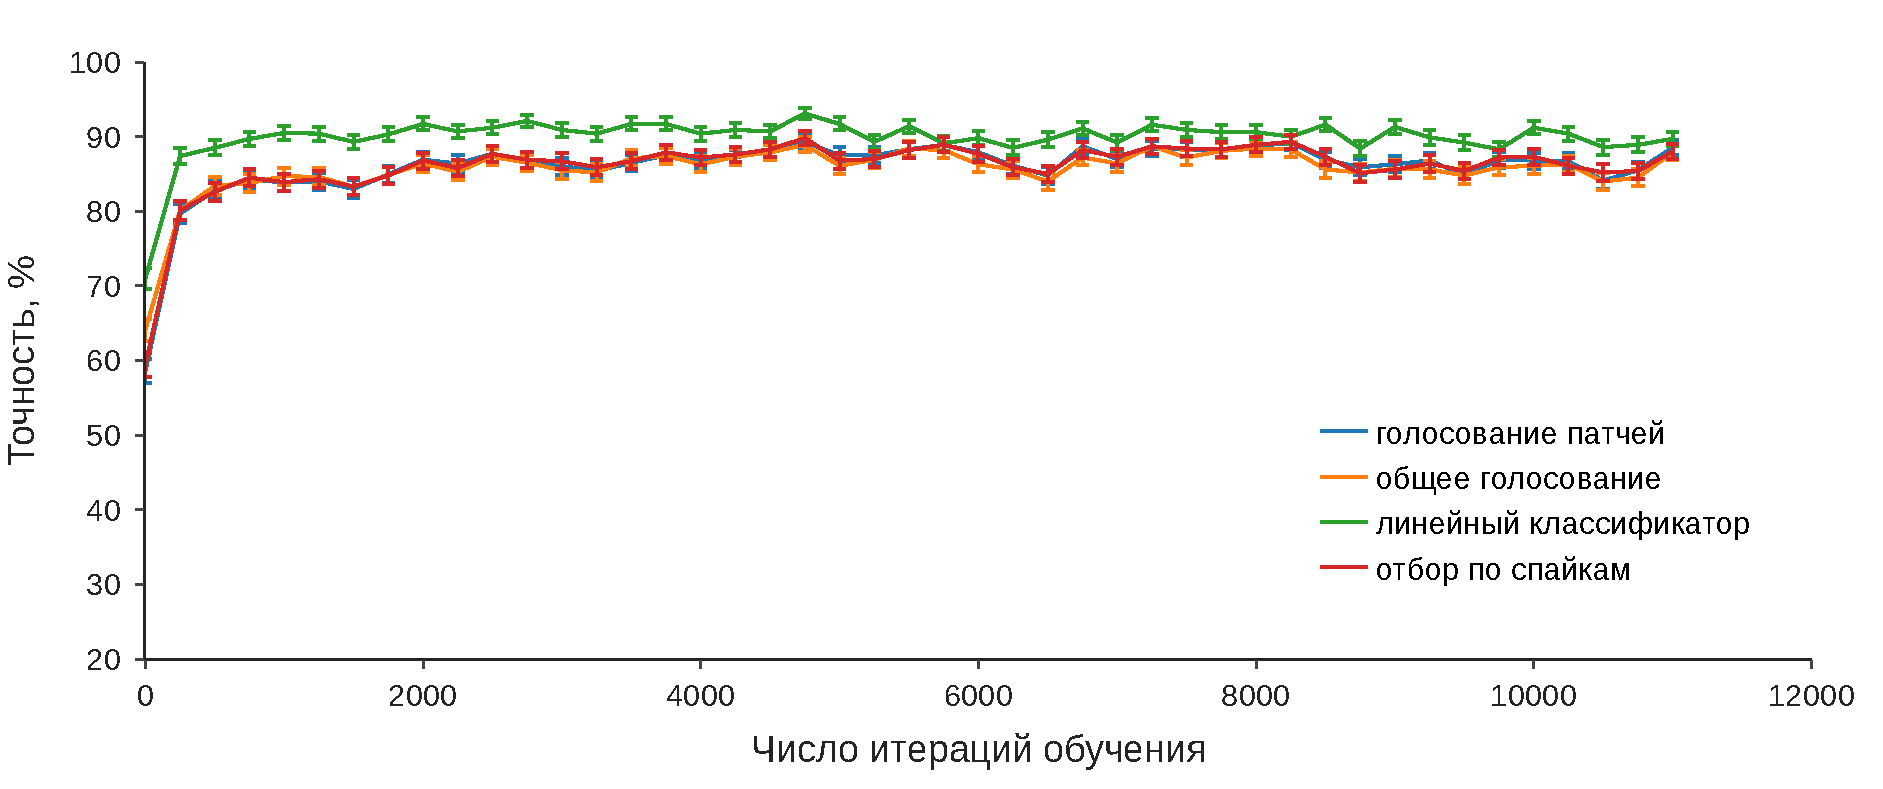
\includegraphics[width=\textwidth,keepaspectratio=true]{LCSNN_learning_rate_ru.pdf}
 \caption{Кривая обучения LCSNN.}
\end{subfigure} 
\begin{subfigure}{\textwidth} 
    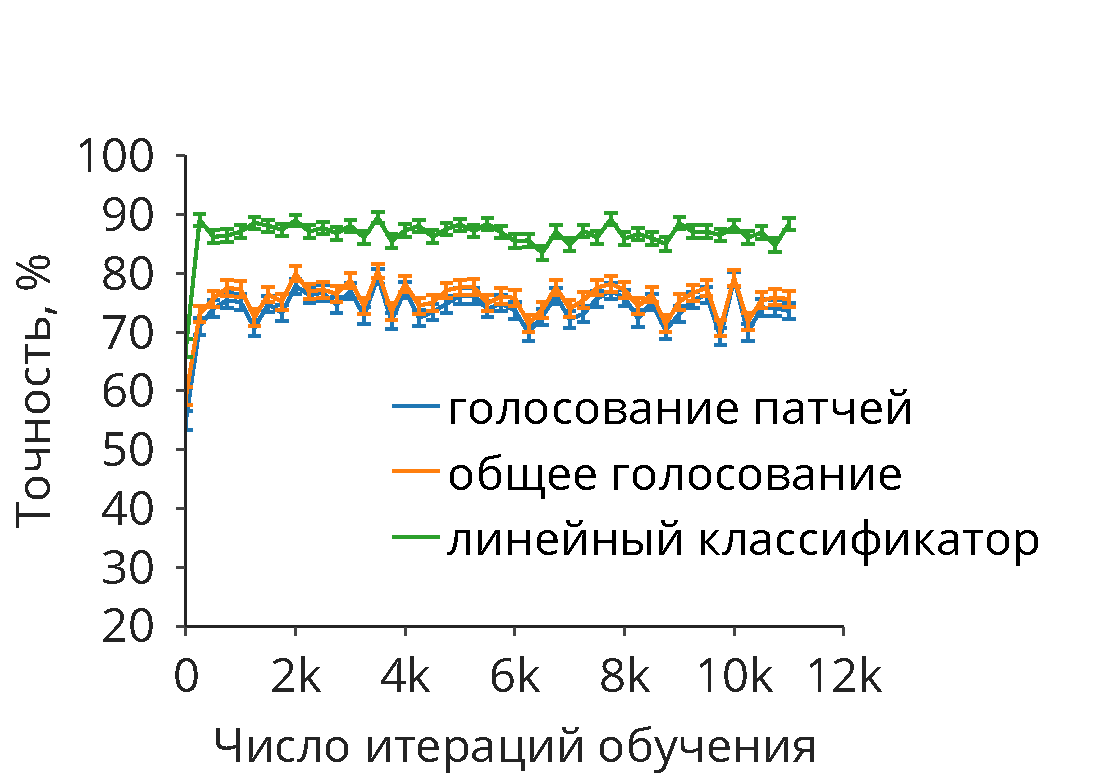
\includegraphics[width=\textwidth,keepaspectratio=true]{CSNN_learning_rate_ru.pdf}
 \caption{Кривая обучения CSNN.}
\end{subfigure}
\end{figure}
\begin{figure}[H]\ContinuedFloat
\begin{subfigure}{\textwidth} 
    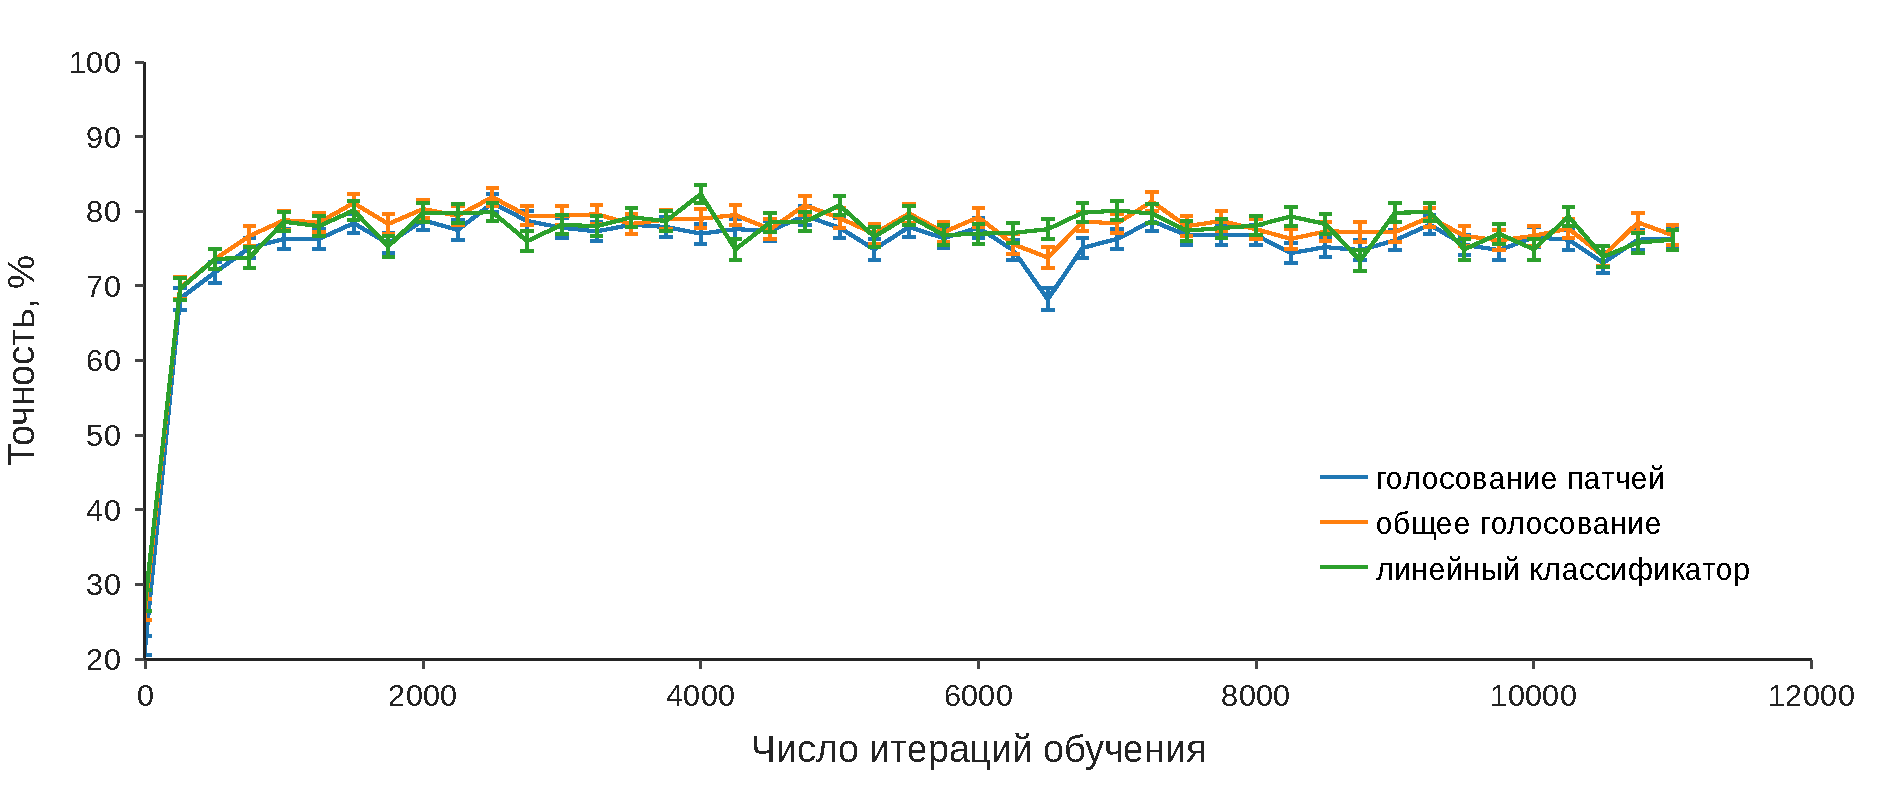
\includegraphics[width=\textwidth,keepaspectratio=true]{FCSNN_learning_rate_ru.pdf}
 \caption{Кривая обучения FCSNN.} 
\end{subfigure}
\caption{Сравнение кривых обучения различных архитектур спайковых нейронных сетей с конкуренцией. Приведены результаты для различных алгоритмов интерпретации активности. Отбор по спайкам проверялся только для LCSNN, потому что практически совпадает по результатам с голосованием патчей. В качестве погрешностей нанесены стандартные отклонения. Все эти сети имеют 100 каналов, размер свертки для LCSNN составляет 12, а для CSNN --- 8.}
\end{figure}

\subsection{Сравнение эффективности операции свертки и локального рецептивного поля}
Были проведены эксперименты по измерению точности сетей с различными архитектурами. Для сверточных и полносвязных сетей вводились аналогичные связи конкуренции. Из-за очень высоких вычислительных нагрузок не ставилось задачи по нахождению параметров, идеально обеспечивающих максимальную точность для каждой архитектуры. Эти параметры были подобраны приблизительно, поэтому могли не попасть в максимум точности, однако величина расхождения не превышает 1-2\%. Все точности посчитаны при помощи алгоритма интерпретации активности на основе голосования нейронов (учитывался лучший результат). Заметим, что при использовании линейного классификатора в качестве алгоритма интерпретации удалось достигнуть 95\% точности для локально соединенной сети из 1000 каналов с размером ядра 12.

\begin{table}[H]
 \caption{Результаты сравнения различных архитектур спайковых нейронных сетей. Для каждой сети точность измерялась $N=5$ раз. В таблице указаны среднее значение и стандартное отклонение для точности.}
\begin{center}
\begin{adjustwidth}{-1cm}{}
\begin{tabular}{|l|l|l|l|l|l|p{2.2cm}|p{2.2cm}|}
\hline
&\multicolumn{5}{c|}{Конфигурация} & \multicolumn{2}{c|}{Точность, \%}\\
\hline
N & Архитектура & Каналы & Ядро & Веса & Нейроны & {Метод \footnotemark[1]} & {Метод \footnotemark[2]} \\
\hline\hline
1 & {LCSNN} & {1000} & {12} & {10287000} & {9000} & {$92.3 \pm 0.7$} & {$95.1 \pm 0.5$}\\
\hline
2 & {LCSNN} & {100} & {12} & {218700} & {900} & {$87.5 \pm 0.9$} & {$91.5 \pm 0.6$}\\
\hline
3 & {LCSNN} & {100} & {8} & {260800} & {1600} & {$82.9 \pm 0.6$} & {$88.1 \pm 0.7$}\\
\hline
{4} & {LCSNN\footnotemark[3]} & {25} & {12} & {37800} & {225} & {$82.3 \pm 1.0$} & \textbf{$88.2 \pm 0.6$}\\
\hline
5 & {LCSNN} & {25} & {12} & {37800} & {225} & {$80.1 \pm 1.0$} & {$85.5 \pm 0.8$}\\
\hline
6 & {LCSNN} & {25} & {8} & {35200} & {400} & {$73.6 \pm 1.0$} & {$80.3 \pm 0.7$}\\
\hline\hline
7 & {CSNN} & {169} & {12} & {255672} & {1521} & {$79.2 \pm 1.6$} & {$85.7 \pm 1.4$}\\
\hline
8 & {CSNN} & {81} & {12} & {58464} & {729} & {$77.2 \pm 1.7$} & {$83.1 \pm 1.2$}\\
\hline
9 & {CSNN} & {100} & {8} & {158464} & {1600} & {$77.4 \pm 1.9$} & {$82.1 \pm 1.3$}\\
\hline
10 & {CSNN} & {25} & {12} & {5544} & {225} & {$65.8 \pm 0.7$} & {$77.1 \pm 0.6$}\\
\hline
11 & {CSNN} & {25} & {8} & {9664} & {400} & {$63.1 \pm 1.2$} & {$75.8 \pm 0.5$}\\
\hline\hline
12 & {FCSNN} & {100} & {20} & {449100} & {100} & {$81.4 \pm 0.9$} & {$82.1 \pm 0.8$}\\
\hline
\end{tabular}
\end{adjustwidth}
\end{center}
 \label{results}
\end{table}

\footnotetext[1]{Лучший алгоритм голосования}
\footnotetext[2]{Линейный классификатор}
\footnotetext[3]{Сеть с обучением связей конкуренции}

Видно (№3 и №7 в таблице \ref{results}), что локально соединенная сеть превосходит сверточную сеть по точности даже при чуть превышающем числе параметров последней. Также видно, что не следует использовать слишком малый размер ядра свертки. Это приводит к выучиванию сетью менее значительных признаков. В классическом машинном обучении используются либо неглубокие сети с большими ядрами свертки, либо глубокие сети с маленькими ядрами свертки.

Заметим, что спайковые нейронные сети могут достигать значительно больших точностей на MNIST. Для этого можно использовать:
\begin{itemize}
\item Сети с существенно большим числом весовых параметров, чем в данной работе (например, увеличив число каналов)
\item Более глубокие сети с большим количеством слоев
\item Другие алгоритмы обучения (например, обучение с учителем)
\end{itemize} 

\begin{table}[H]
 \caption{Результаты других исследований спайковых нейронных сетей. Во всех используется датасет MNIST.}
\begin{center}
\begin{tabular}{|l|p{4cm}|p{7cm}|l|l|}
\hline
Статья & Архитектура & Обучение & Точность, \% \\
\hline\hline
{Эта работа} & {Локальная + конкуренция} & {Без учителя} & {$95.1 \pm 0.5$}\\
\hline\hline
{\cite{saunders2019locally}} & {Локальная + конкуренция} & {Без учителя} & {$95.07 \pm 0.63$}\\
\hline
{\cite{mnist2}} & {Полносвязная + конкуренция} & {Без учителя} & {95}\\
\hline
{\cite{MaxActiv1}} & {Полносвязная + конкуренция} & {С учителем / с частичным привлечением учителя} & {95.4 / 72.1}\\
\hline
{\cite{conv1}} & {Сверточная} & {С частичным привлечением учителя} & {$96.95 \pm 0.08$}\\
\hline
{\cite{conv2}} & {Сверточная} & {С частичным привлечением учителя} & {$99.28 \pm 0.10$}\\
\hline
{\cite{conv3}} & {Сверточная} & {С частичным привлечением учителя} & {$97.20 \pm 0.07$}\\
\hline
\end{tabular}
\end{center}
\end{table}

Результат, полученный в настоящей работе, практически соответствует результату из \cite{saunders2019locally}. Заметим, что при помощи признаков, обученных без учителя достигаются результаты, лишь немногим уступающие результатам, полученным при помощи обучения с учителем. При этом лучшая локально соединенная сеть с конкуренцией локальных рецептивных полей из этой работы имеет $10^7$ связей (из них связей прямого распространения --- $1 \cdot 10^6$, связей конкуренции --- $9 \cdot 10^6$), по сравнению с $4.6 \cdot 10^7$ (из них связей прямого распространения --- $0.5 \cdot 10^7$, связей конкуренции --- $4.1 \cdot 10^7$) у полносвязной сети с конкуренцией из \cite{mnist2}. К тому же, обучение сети из \cite{mnist2} велось в течение $1 \cdot 10^6$ итераций, тогда как в этой работе число итераций обучения не превосходит 5000.

\section{Обучение связей конкуренции}
Связи $YY$ существенно влияют на обучение связей $XY$. Большие по модулю значения способствуют вариативности в обучении $Y$ нейронов, так для каждого рецептивного поля одновременно активными не могут быть нейроны, имеющие схожие веса $XY$. Малые по модулю значения не позволяют нейронам специализироваться. 

Примечательно, что с такими большими по модулю значениями весов конкуренции для каждого рецептивного поля остается активным лишь один нейрон (или реже несколько нейронов), веса которого лучше всего соответствует области представленного изображения, который подавляет активность остальных.

% \begin{figure}[H]
% \centering
% \begin{subfigure}{0.95\textwidth} 
%     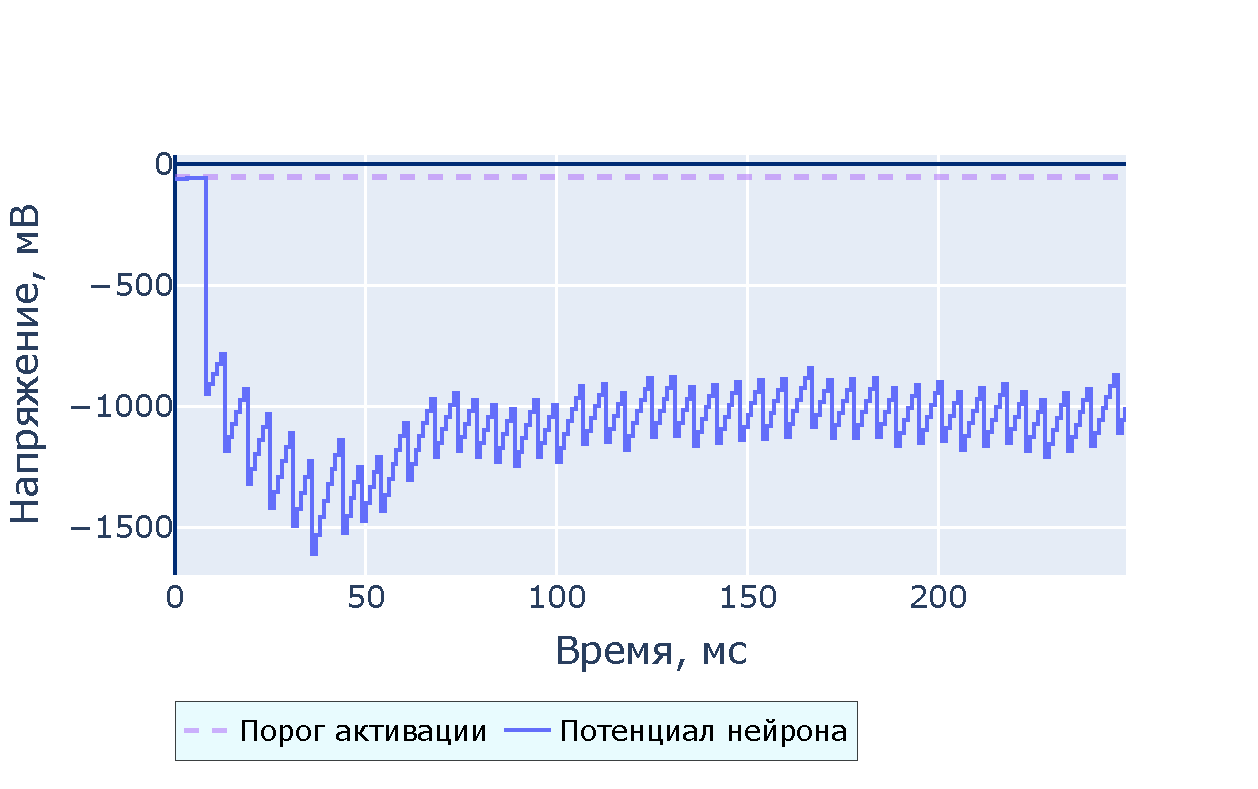
\includegraphics[width=\textwidth,keepaspectratio=true]{bad_voltage_ru.pdf}
%     \caption{Активность нейрона, который проиграл в конкуренции, подавлена другими нейронами.
%     } 
% \end{subfigure}
% \begin{subfigure}{0.95\textwidth}
%     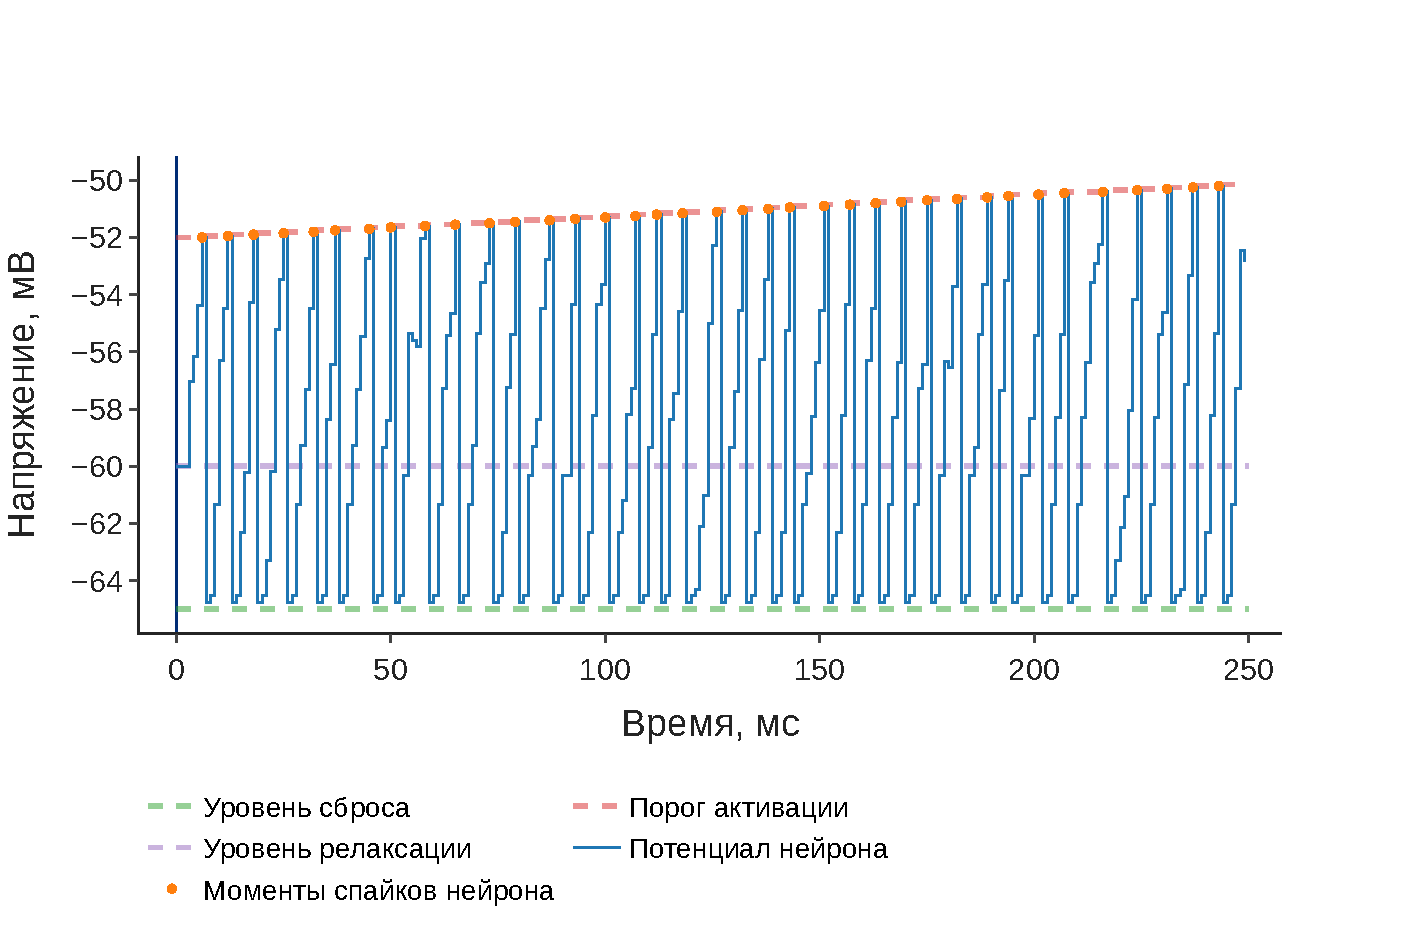
\includegraphics[width=\textwidth,keepaspectratio=true]{good_voltage_ru.pdf}
%     \caption{Активность нейрона, который выиграл в конкуренции. Присутствуют множество спайков.}
% \end{subfigure}
% \caption{Влияние конкуренции на активность нейронов\\
% \textit{Примечание: на графике слева не представлены значения $v_{rest}$ и $v_{reset}$, так как на данном масштабе они практически совпадают с $v_{thresh}$.}
% }
% \end{figure} 

\begin{figure}[H]
\centering
\begin{subfigure}{0.45\textwidth}
    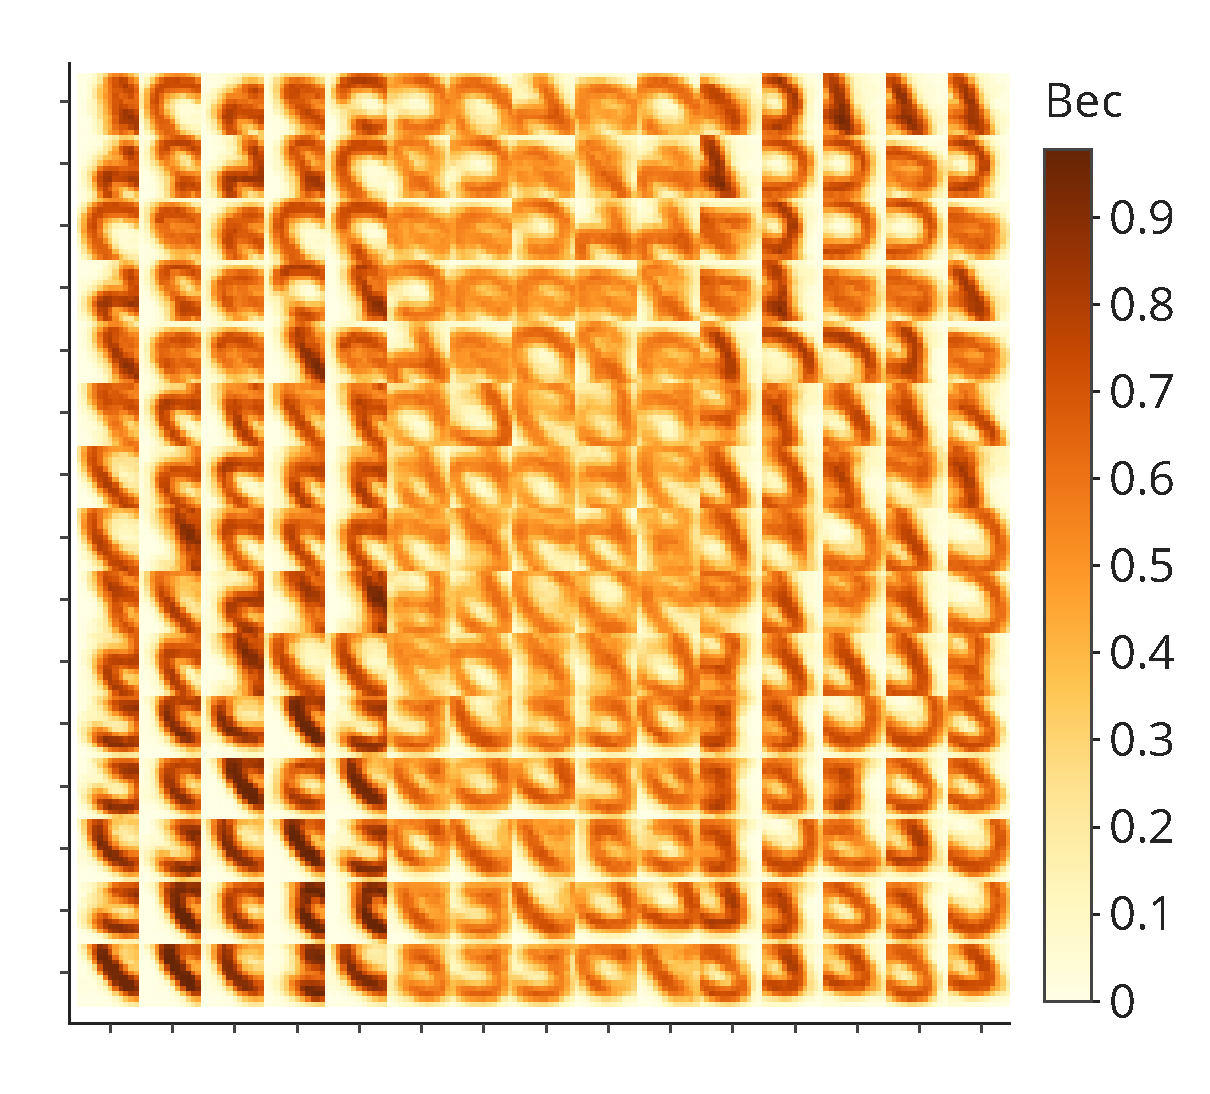
\includegraphics[width=\textwidth,keepaspectratio=true]{weights_XY_bad_ru.pdf}
    \caption{Слабо специализированные веса,\\ вес конкуренции равен --10.}
\end{subfigure}
\begin{subfigure}{0.45\textwidth}
    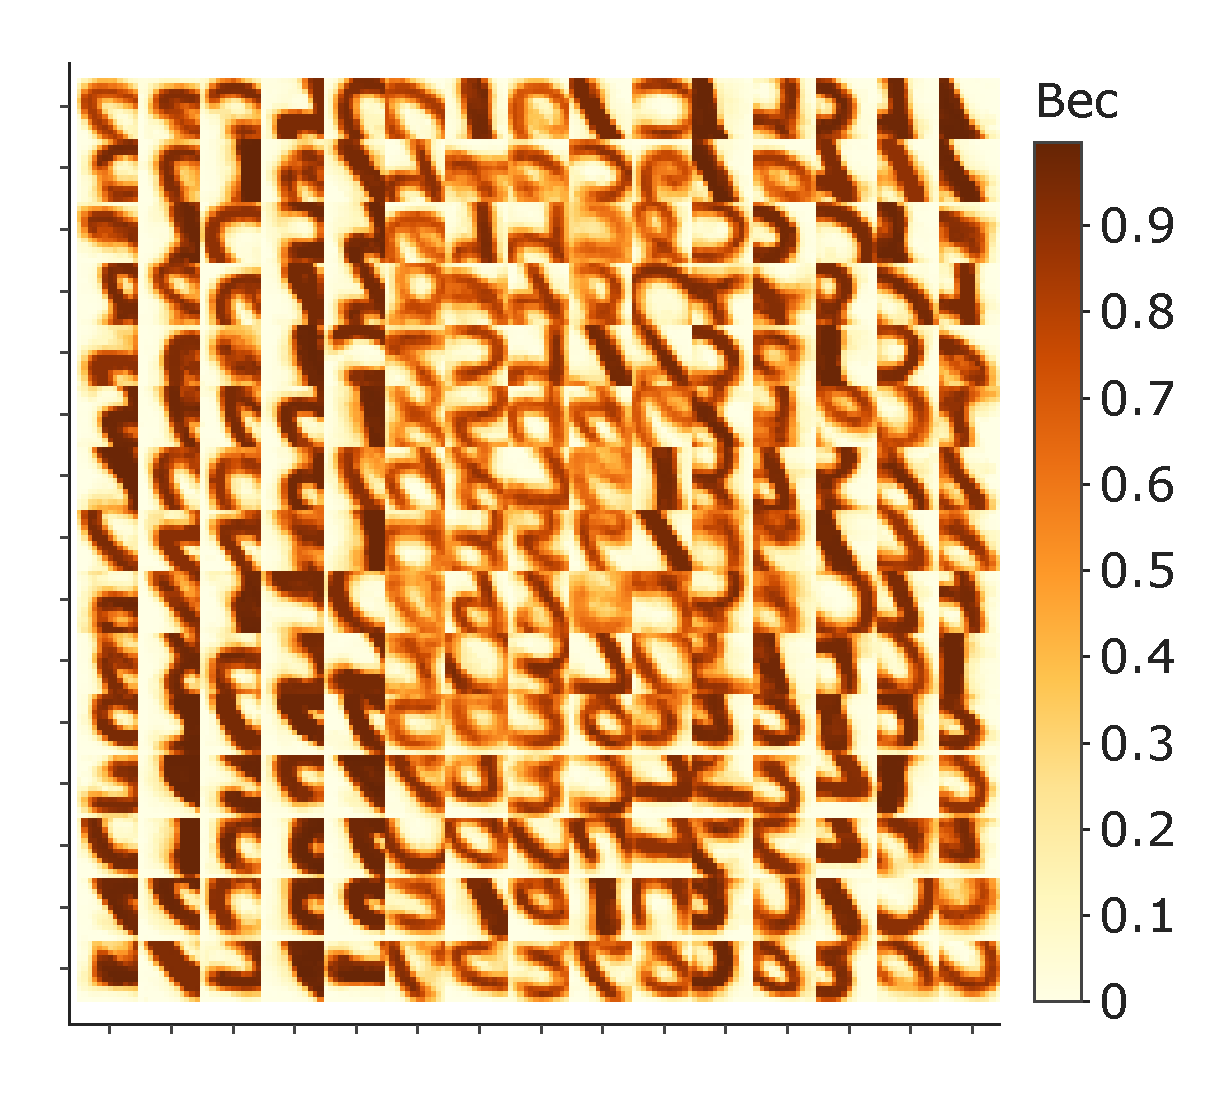
\includegraphics[width=\textwidth,keepaspectratio=true]{weights_XY_good_ru.pdf}
    \caption{Высоко специализированные веса,\\ вес конкуренции равен --100.}
\end{subfigure}
\caption{Влияние конкуренции на обучение связей $XY$.}
\label{competition-training-importance}
\end{figure}

Все сети, о которых шла речь до этого в работе, имели фиксированные веса конкуренции. Было обнаружено, что обучение весов конкуренции позволяет повысить точность сети. Для обучения связей $YY$ используется правило anti-STDP (правило, обратное STDP знаками $A_{+}$ и $A_{-}$). При помощи варьирования параметров этого правила были получены различные распределения весов конкуренции.

\begin{figure}[H]
\centering
\begin{subfigure}{0.45\textwidth}
    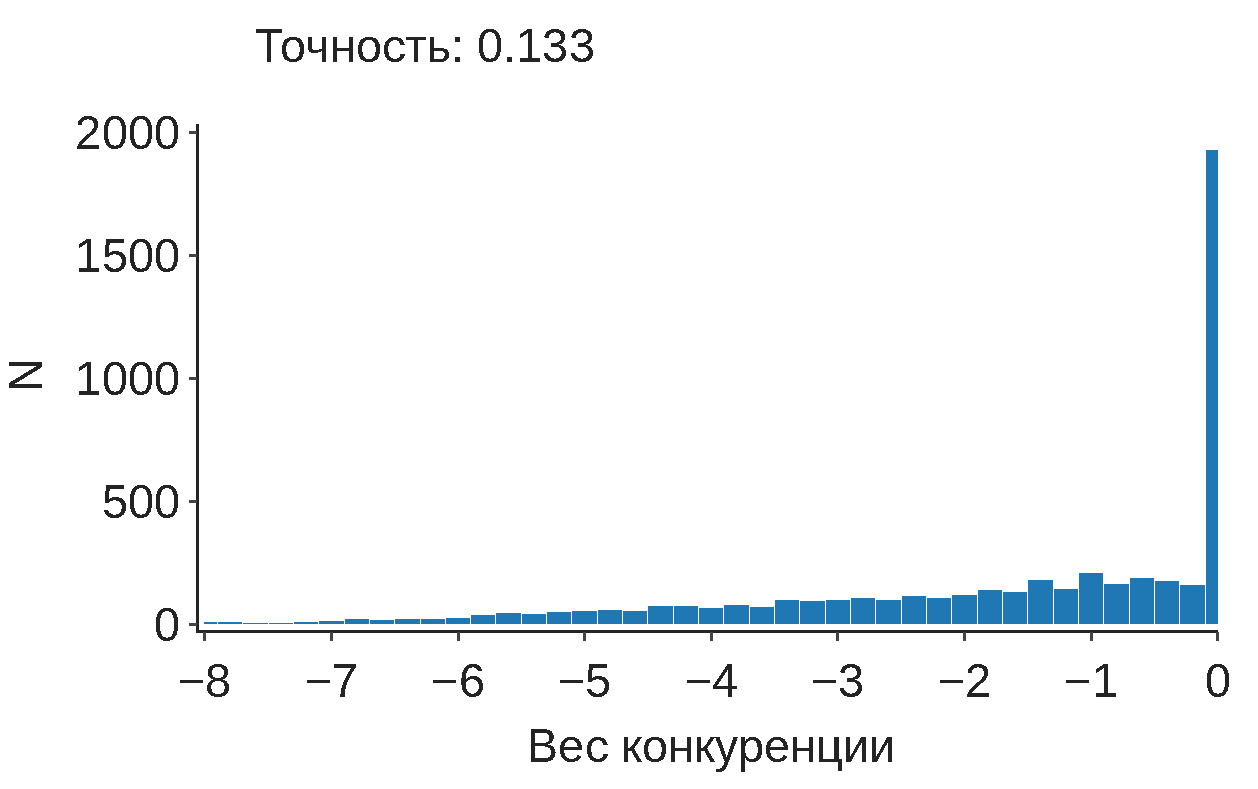
\includegraphics[width=\textwidth,keepaspectratio=true]{competition_distribution_worst_ru.pdf}
    \caption{Очень слабая конкуренция}
\end{subfigure}
\begin{subfigure}{0.45\textwidth}
    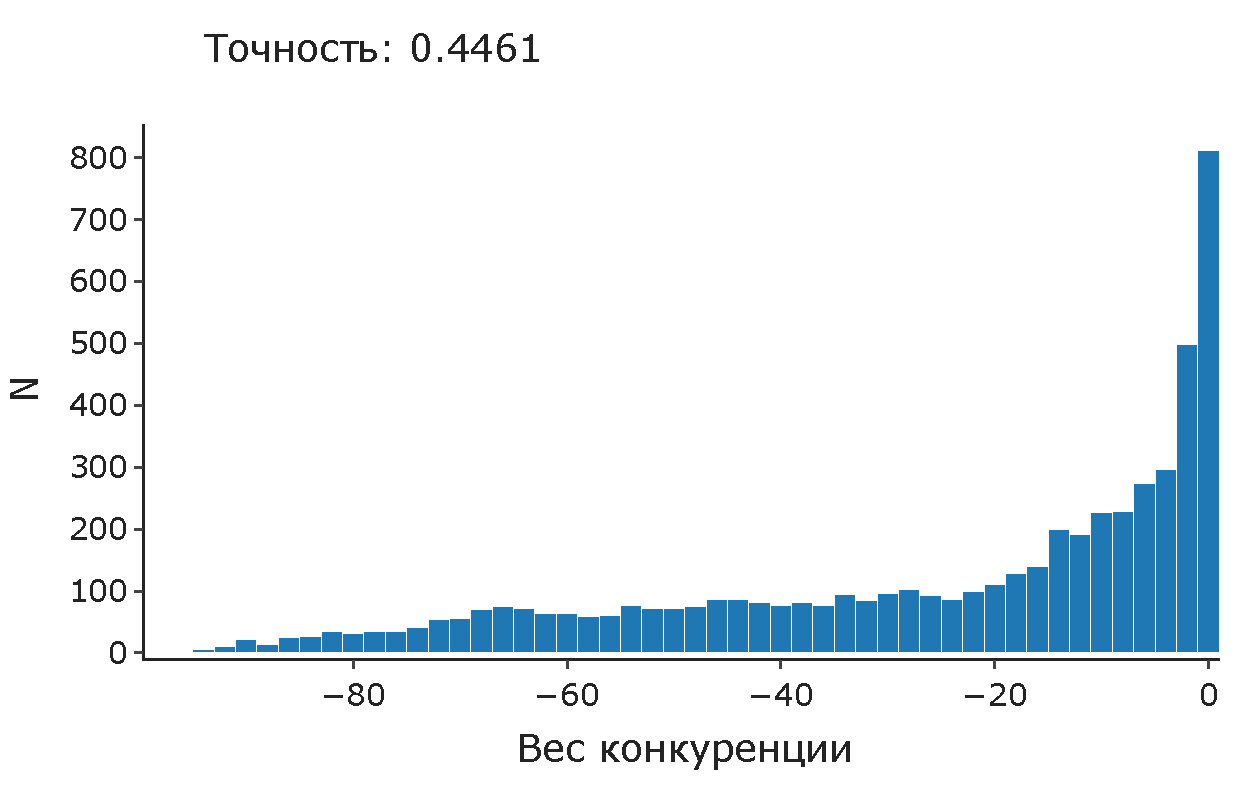
\includegraphics[width=\textwidth,keepaspectratio=true]{competition_distribution_medium_bad_ru.pdf}
    \caption{Слабая конкуренция}
\end{subfigure}
\\
\begin{subfigure}{0.45\textwidth}
    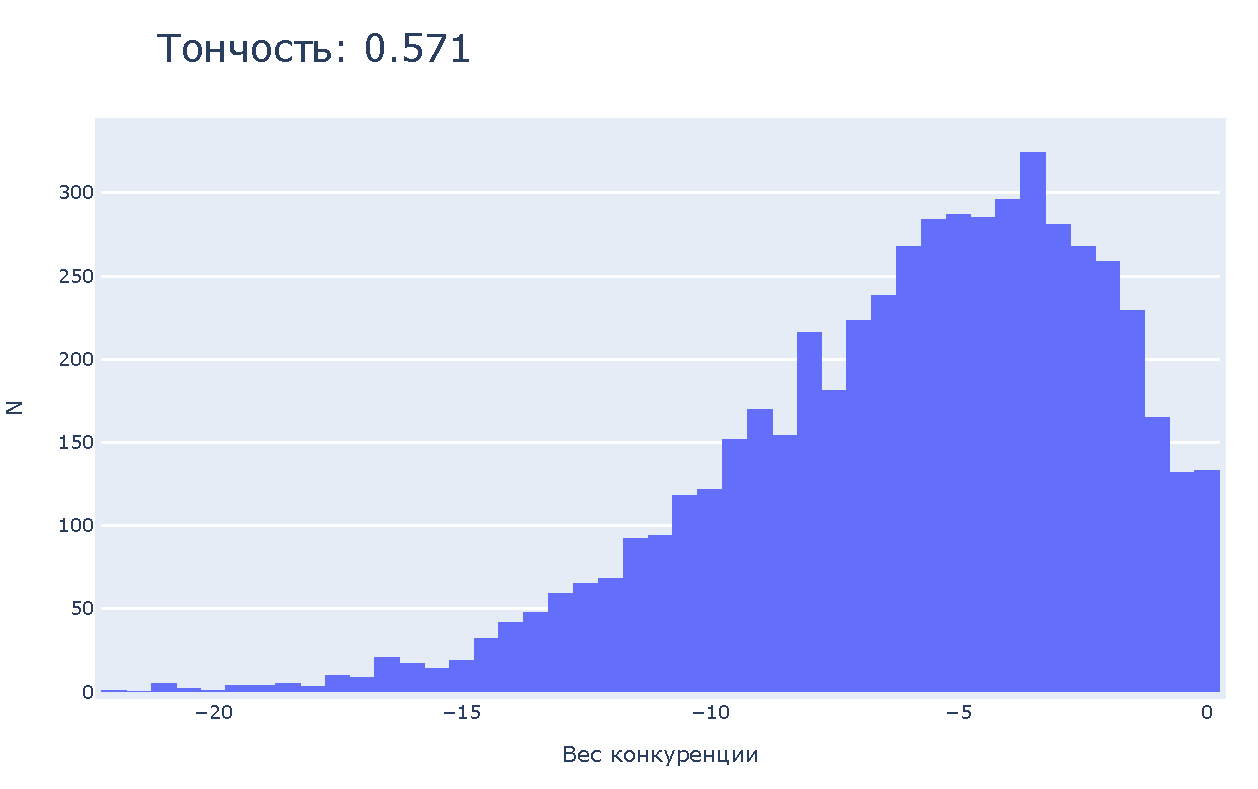
\includegraphics[width=\textwidth,keepaspectratio=true]{competition_distribution_medium_good_ru.pdf}
    \caption{Средняя конкуренция} 
\end{subfigure}
\begin{subfigure}{0.45\textwidth}
    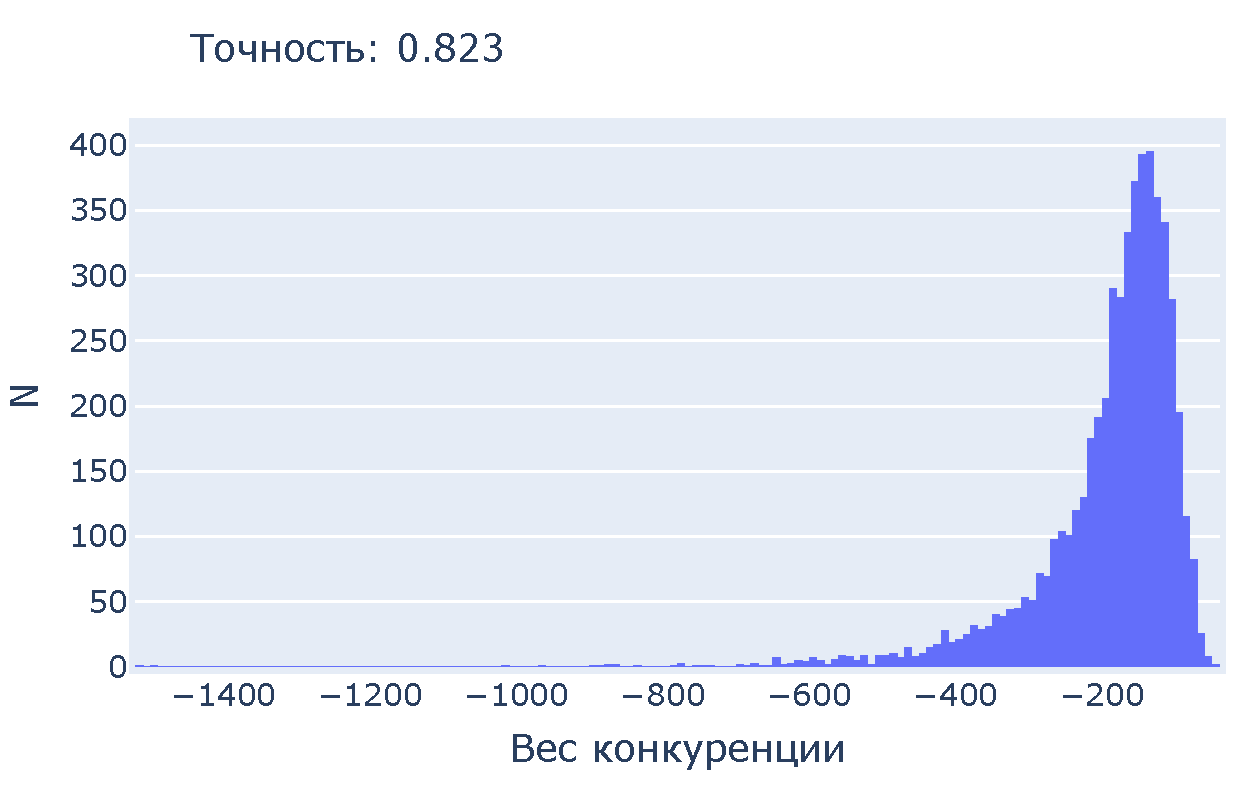
\includegraphics[width=\textwidth,keepaspectratio=true]{competition_distribution_best_ru.pdf}
    \caption{Сильная конкуренция}
    \label{fig:best_competition}
\end{subfigure}
\caption{Различные распределения весов конкуренции}
\label{fig:competition_distributions}
\end{figure}

Видно, что точность сети повышается при тяготении распределения весов конкуренции в сторону больших по модулю значений. Заметим, что целью являлось не нахождение параметров сети, обеспечивающих максимальную точность, а исследования влияния способности обучения конкуренции на точность сети с заданной конфигурацией остальных параметров.

Примечательно, что не все связи $YY$ получают большие по модулю значения. Это объясняется тем, что нейроны, специализирующиеся на значительно разных признаках, не нуждаются в конкуренции, так как они не проявляют высокую активность одновременно.

\begin{figure}[H]
\centering
\begin{subfigure}{0.45\textwidth} 
    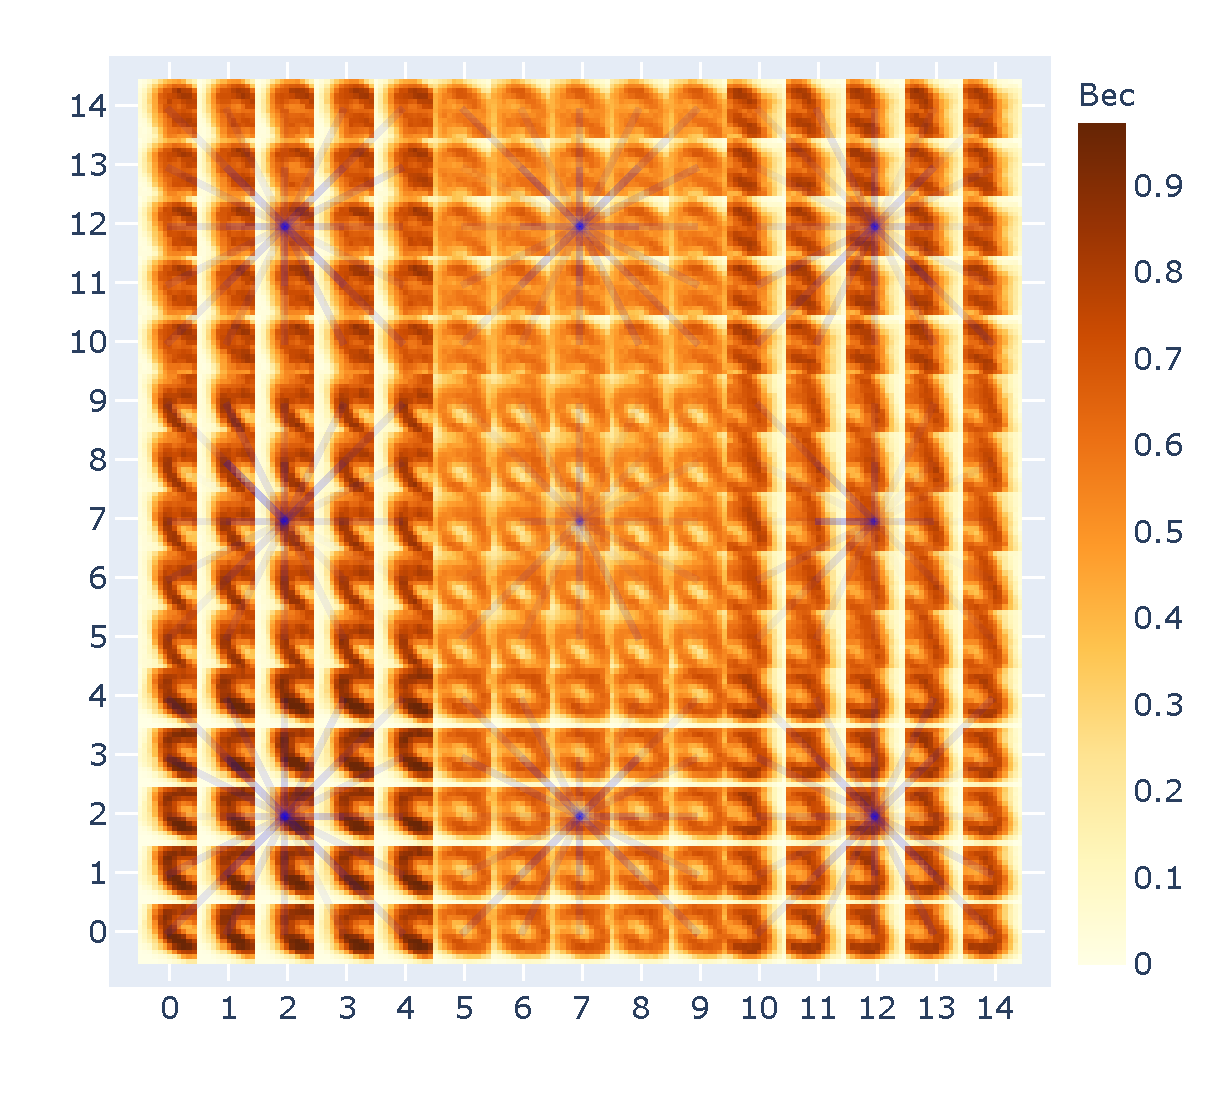
\includegraphics[width=\textwidth,keepaspectratio=true]{competition_on_XY_worst_ru.pdf}
    \caption{Очень слабая конкуренция}
\end{subfigure}
\begin{subfigure}{0.45\textwidth}
    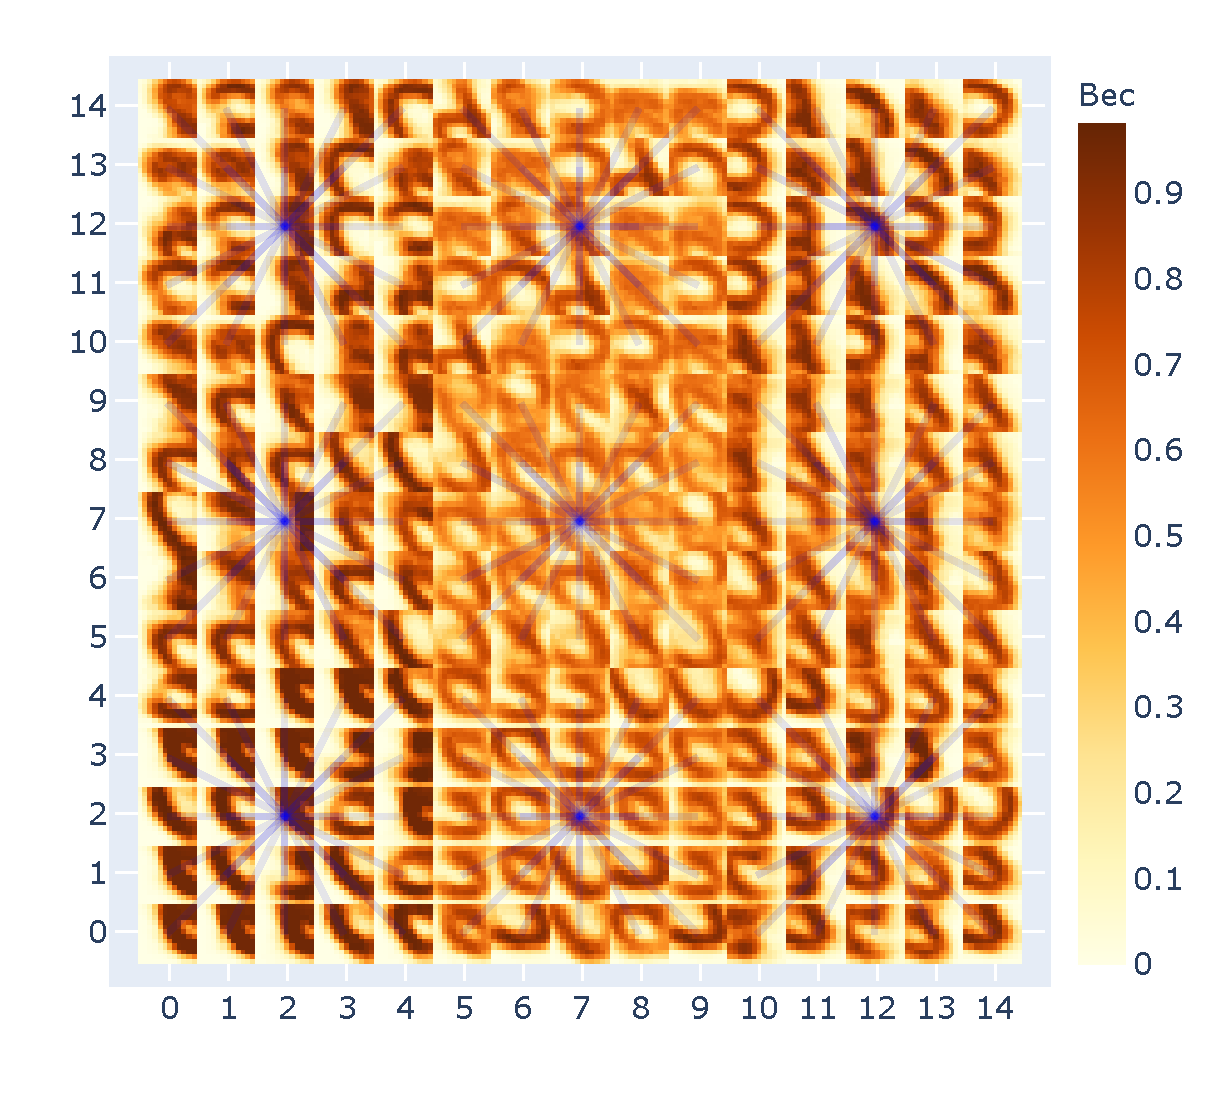
\includegraphics[width=\textwidth,keepaspectratio=true]{competition_on_XY_medium_bad_ru.pdf}
    \caption{Слабая конкуренция}
\end{subfigure}
\\
\begin{subfigure}{0.45\textwidth}
    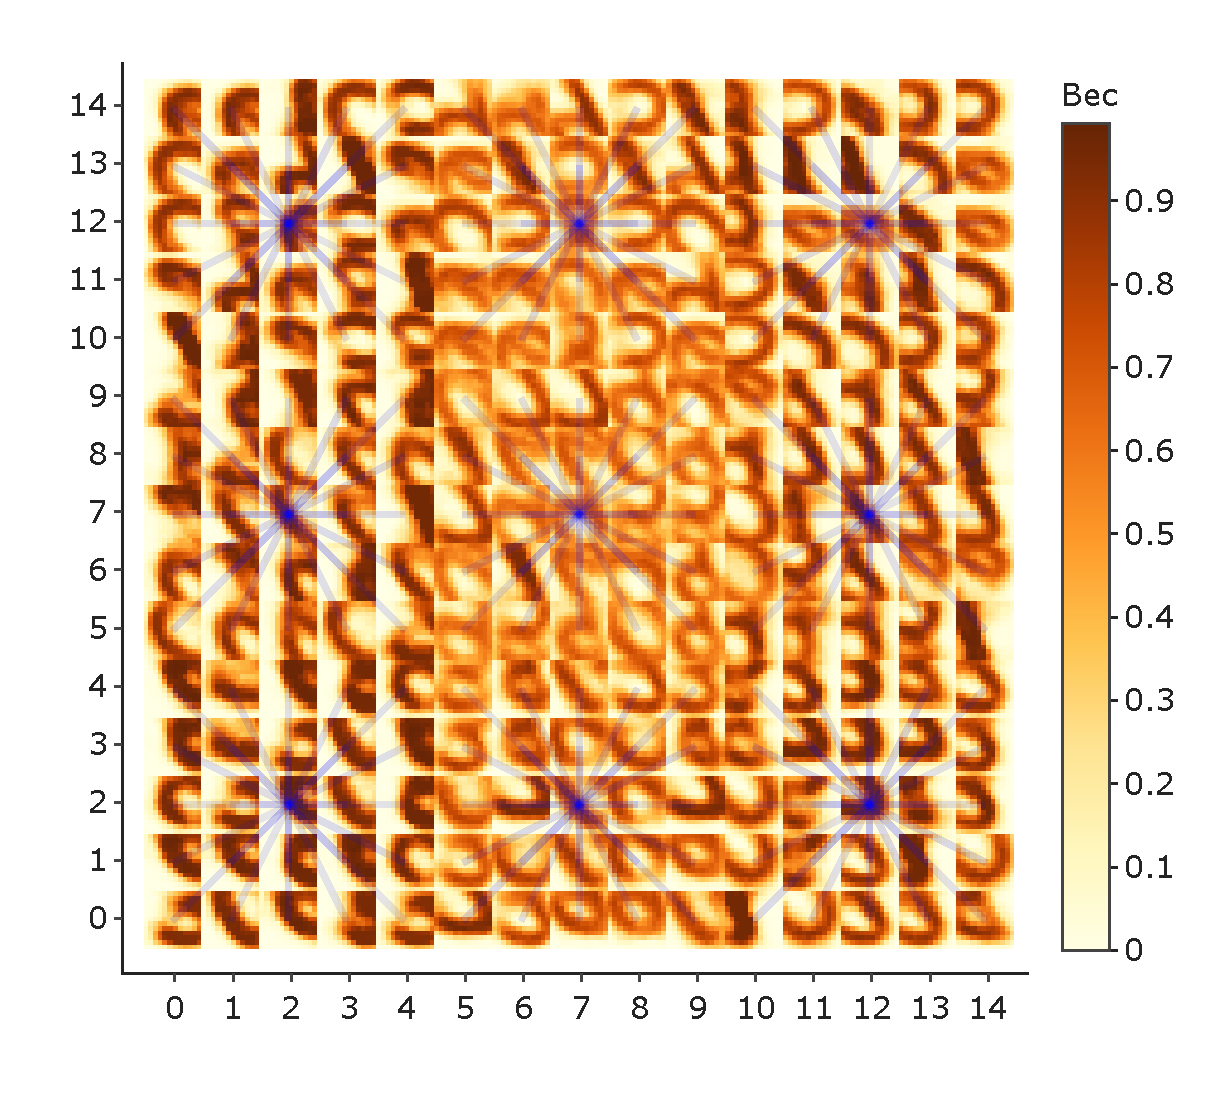
\includegraphics[width=\textwidth,keepaspectratio=true]{competition_on_XY_medium_good_ru.pdf}
    \caption{Средняя конкуренция}
\end{subfigure}
\begin{subfigure}{0.45\textwidth} 
    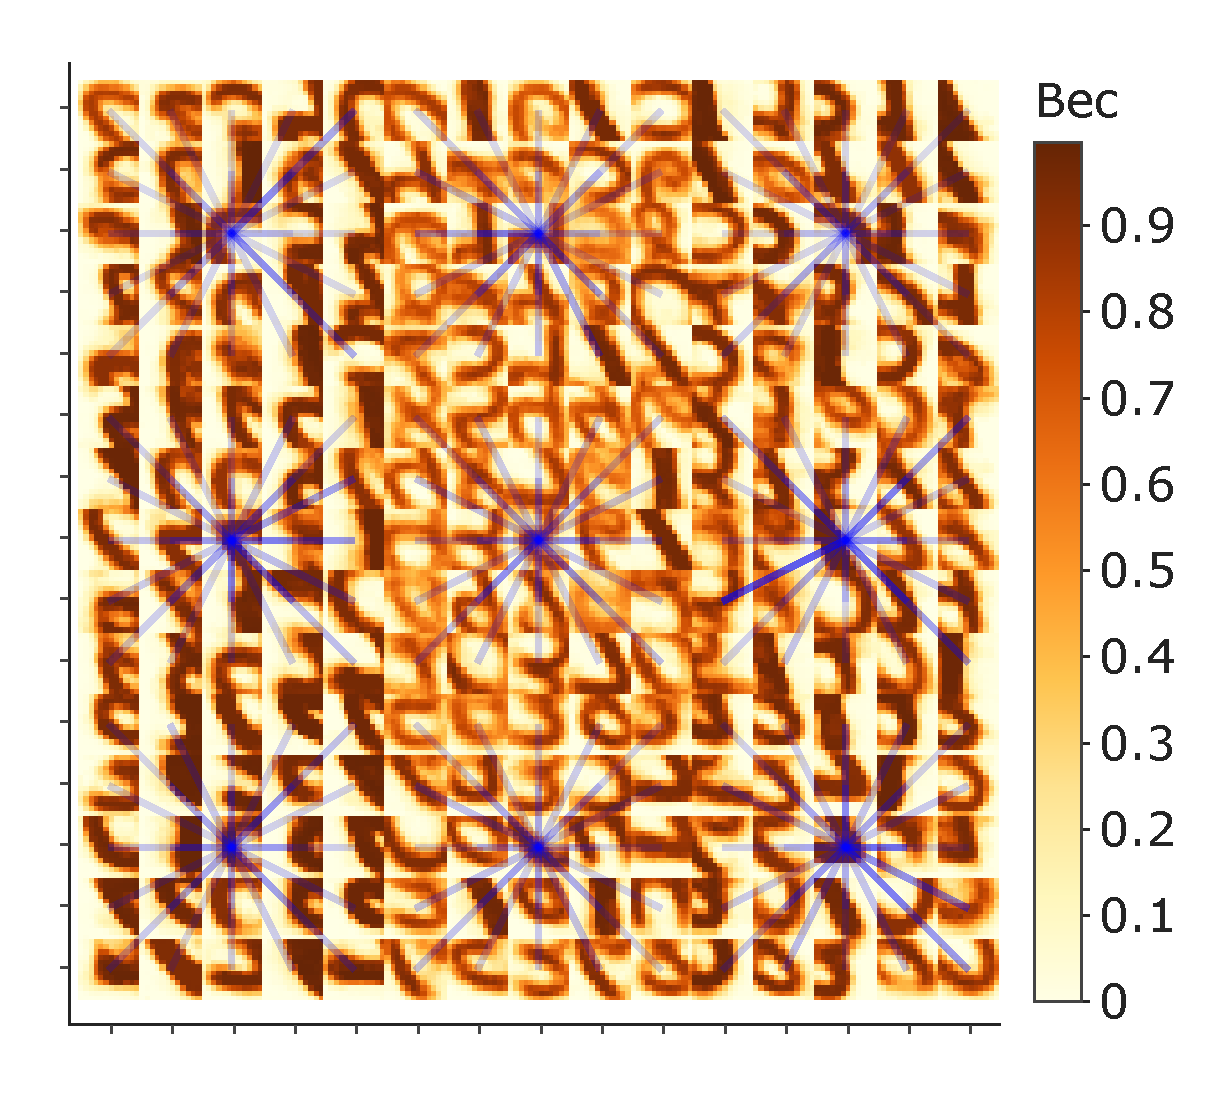
\includegraphics[width=\textwidth,keepaspectratio=true]{competition_on_XY_best_ru.pdf}
    \caption{Сильная конкуренция}
    \label{fig:best_competition_XY}
\end{subfigure}
\caption{Визуализация весов конкуренции поверх весов $XY$. Изображения соответствуют весам сетей с рисунка \ref{fig:competition_distributions}. Изображены только веса конкуренции для одного нейрона в каждом рецептивном поле для избегания загромождения визуализации. Насыщенный синий цвет соответствует большей по модулю конкуренции (используется среднее арифметическое между весами $W_{ij}$ и $W_{ji}$). Видно, что похожие признаки сильнее конкурируют между собой, чем различные.} 
\end{figure}

В ходе оптимизации моделей была измерена точность большого количества сетей со различными конфигурациями гиперпараметров. Оказалось, что не существует четкого интервала ни для среднего веса нормировки (определяющего средний $XY$ связей для каждого $Y$ нейрона), для начального веса конкуренции, ни для параметров anti-STDP для обучения $YY$ связей, который обеспечивал бы высокую точность классификации в не зависимости от значений других гиперпараметров. Это означает, что для максимизации точности не обязательно выбирать определенные значения этих гиперпараметров. Напротив, некоторые из них можно задать практически произвольно, а остальные подобрать. Это ценное наблюдение для реализации связей конкуренции на аппаратной основе.

\begin{figure}[H] \label{fig:hyperparams} 
\begin{center} 
 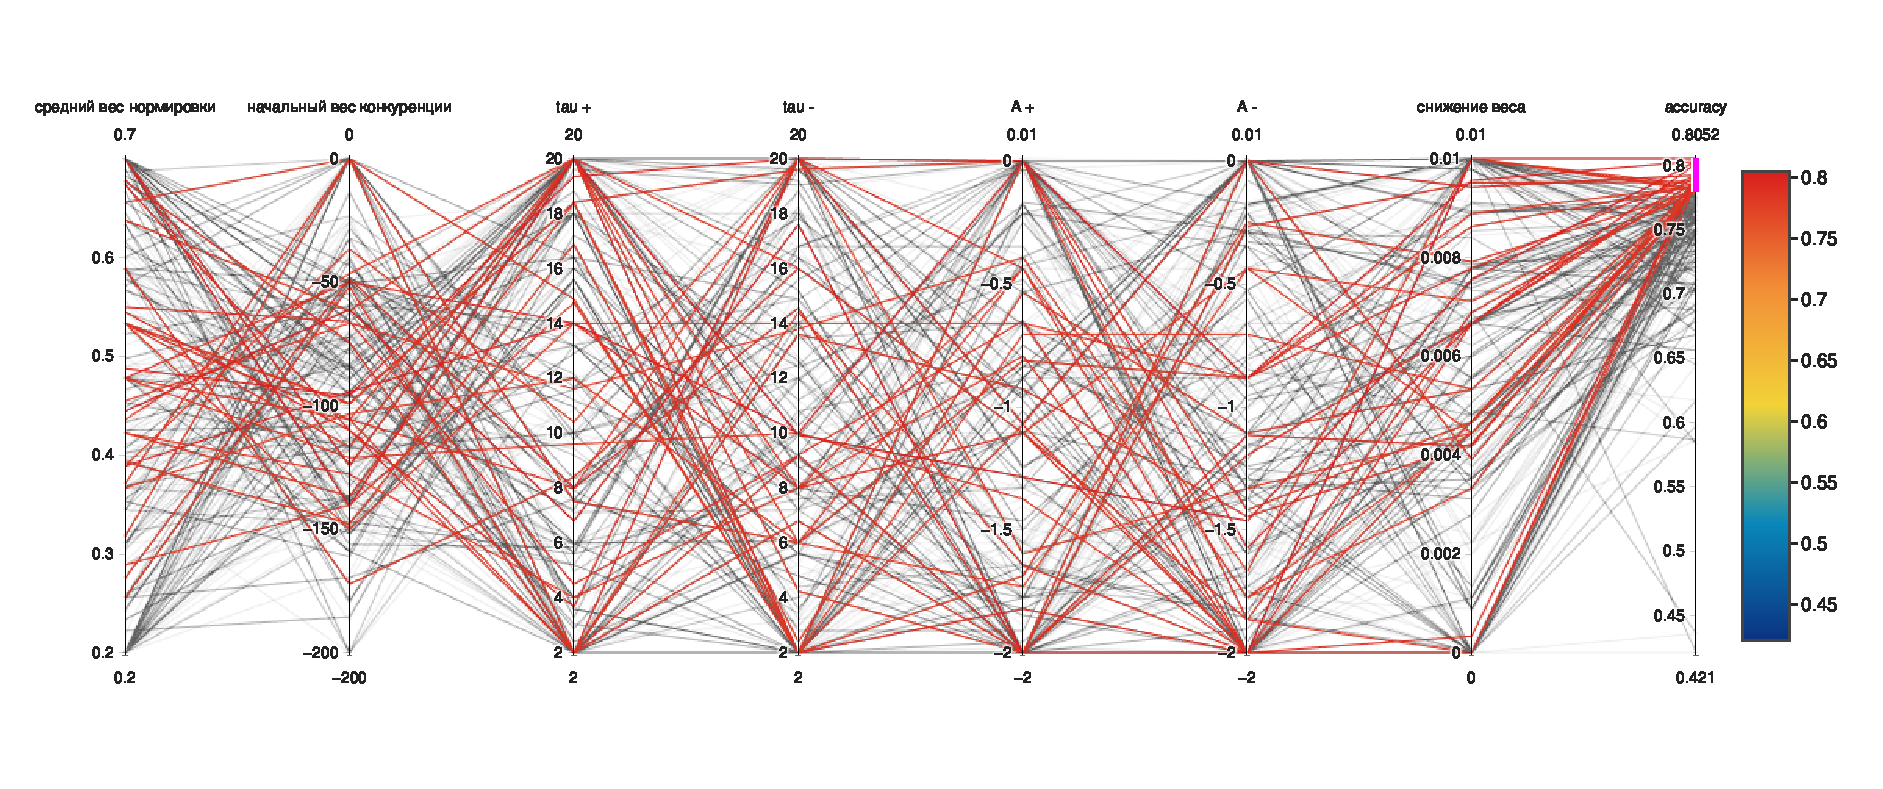
\includegraphics[,
 width=\textwidth,keepaspectratio=true]{hyperparams_ru.pdf}
 
 \caption{Визуализация проверенного пространства гиперпараметров. 1,2 и 7 отвечают за значения весов, 3-6 - параметры anti-STDP. На последней оси указана точность сети с конфигурацией, соответствующей ломаной, проходящей через свои значения гиперпараметров. Видно, что ни на одной из осей нет области сосредоточения ломаных с высокой точностью (выделены красным).}
\end{center}
\end{figure}

\subsection{Анализ обученных весов конкуренции}
Были проведены эксперименты по ограничению значений весов конкуренции сверху и снизу. Оказалось, что как небольшие по модулю, так и большие по модулю веса конкуренции играют важную роль в работе сети, так как ограничение как сверху, так и снизу отрицательно влияет на точность распознавания. Это объясняется тем, что высокая конкуренция способствует большей специализации нейронов - и потому полезна, а низкая конкуренция позволяет нейронам кооперироваться и распознавать классы вместе (в том числе накапливая большую статистику для калибровки).

\begin{figure}[H] 
\centering
% \begin{subfigure}{0.70\textwidth}
%     \includegraphics[width=\textwidth,keepaspectratio=true]{competition_distribution_clamp_base_ru.pdf}
%     \caption{Слабая конкуренция}
% \end{subfigure} 

\begin{subfigure}{0.45\textwidth}
    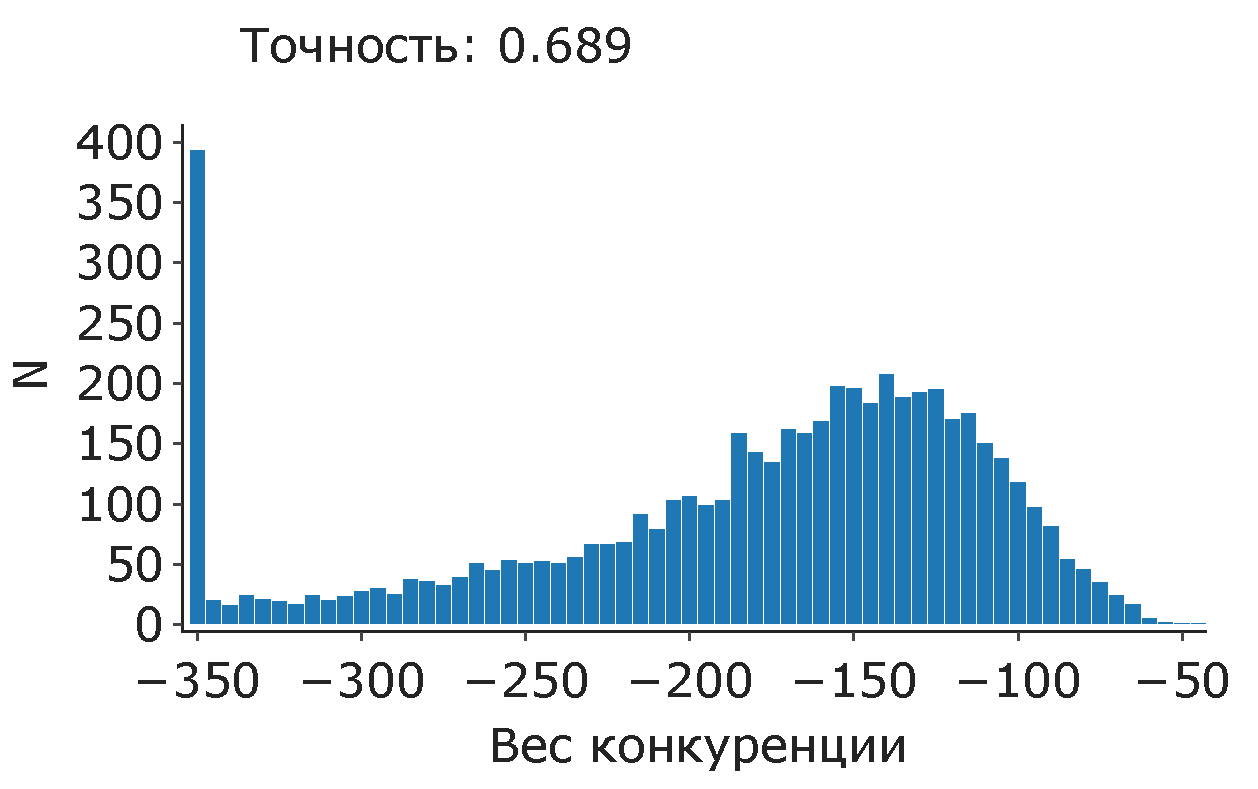
\includegraphics[width=\textwidth,keepaspectratio=true]{competition_distribution_clamp_low_ru.pdf}
    \caption{Распределение весов конкуренции, ограничение сверху} 
\end{subfigure}
\begin{subfigure}{0.45\textwidth}
    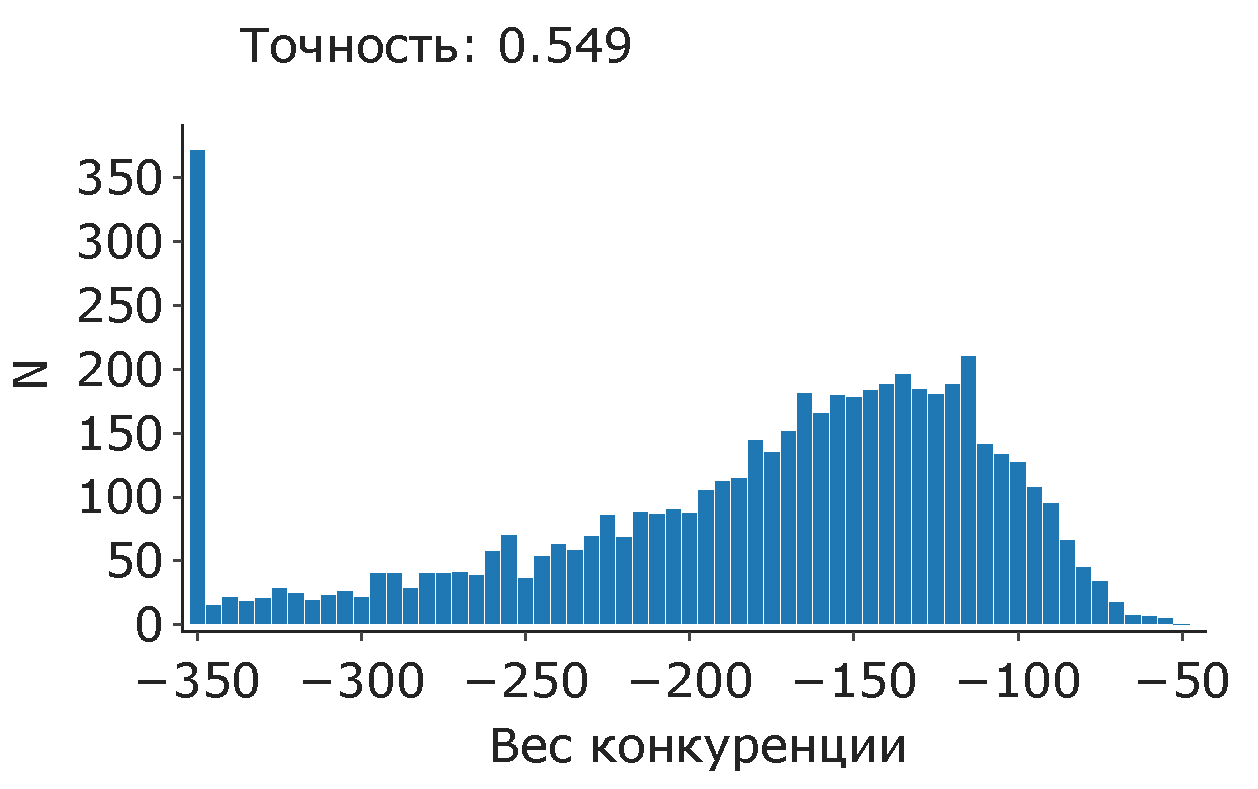
\includegraphics[width=\textwidth,keepaspectratio=true]{competition_distribution_clamp_high_ru.pdf}
    \caption{Распределение весов конкуренции, ограничение снизу}
\end{subfigure}
\begin{subfigure}{0.45\textwidth}
    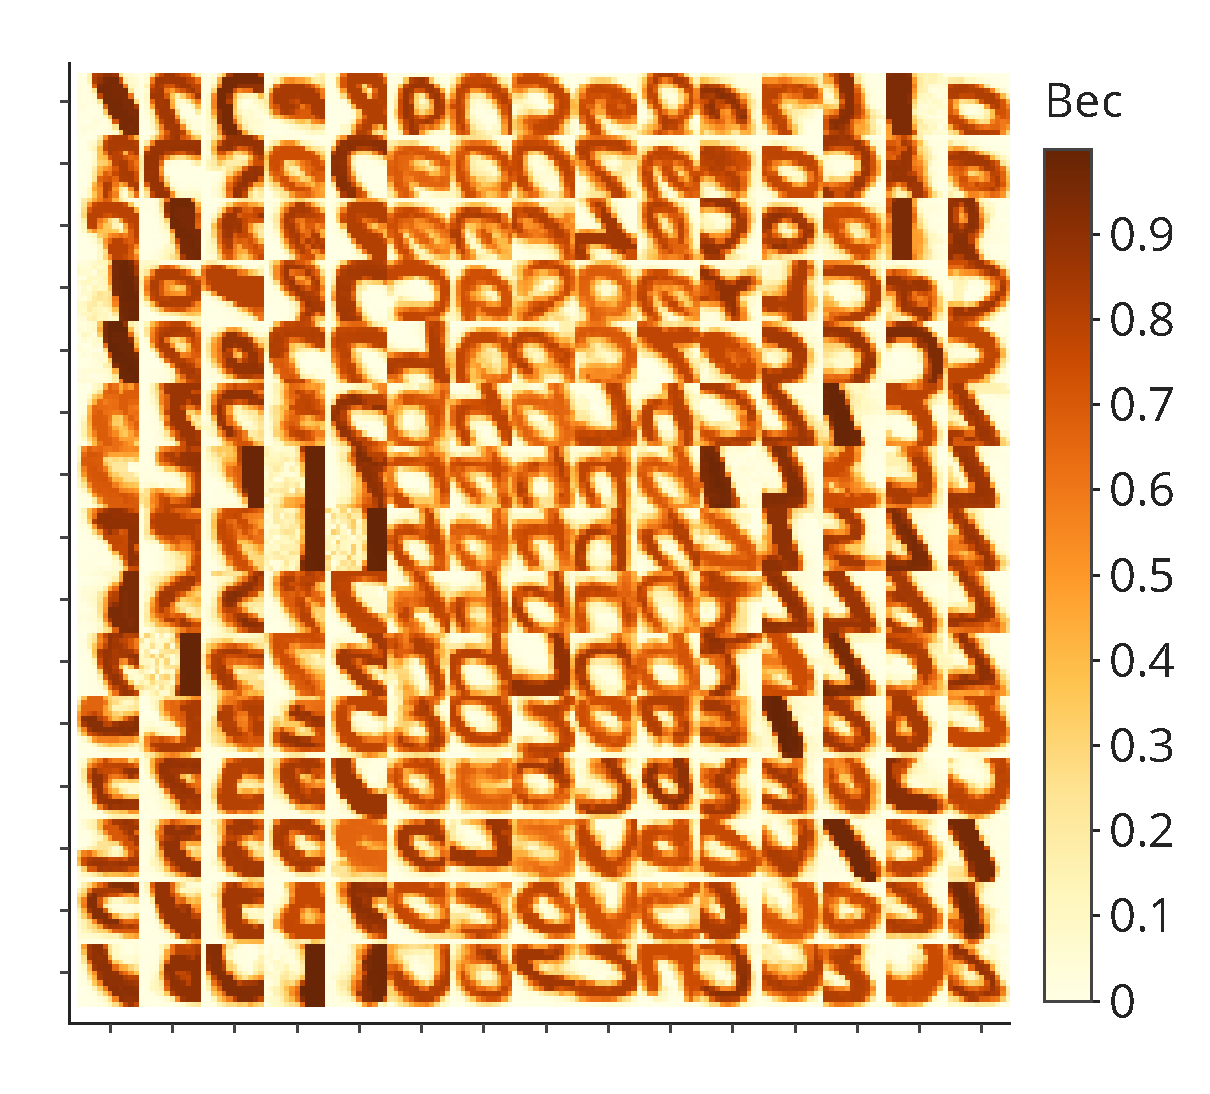
\includegraphics[width=\textwidth,keepaspectratio=true]{weights_XY_clamp_low_ru.pdf}
    \caption{Веса прямого распространения, ограничение сверху}
\end{subfigure} 
\begin{subfigure}{0.45\textwidth}
    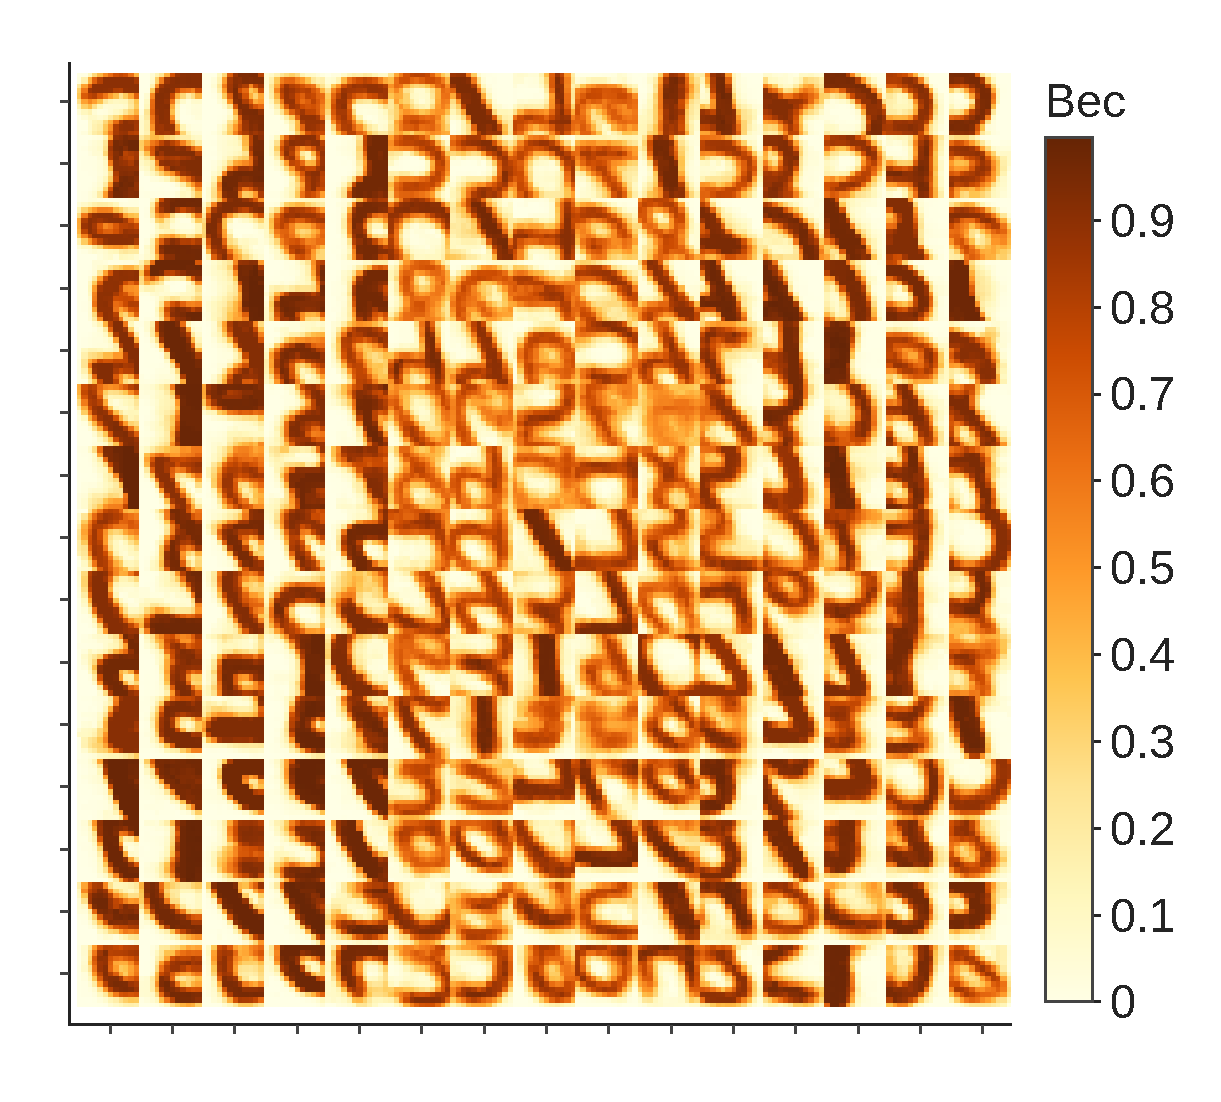
\includegraphics[width=\textwidth,keepaspectratio=true]{weights_XY_clamp_high_ru.pdf}
    \caption{Веса прямого распространения, ограничение снизу}
\end{subfigure} 
\caption{Влияние ограничения значений весов конкуренции на точность. Веса были ограничены значениями $-350$ снизу и $-100$ сверху. Точность сети с аналогичными параметрами, но без ограничения конкуренции составляет 0.823, ее веса $XY$ изображены на Рис. \ref{fig:best_competition_XY}, а распределение ее весов конкуренции --- на Рис. \ref{fig:best_competition}. Видно, что в обоих случаях обучаются менее четкие веса прямого распространения.}
\end{figure}

Обучение конкуренции позволило достичь точности, незначительно (на 2\%) превышающей точность сети такой же конфигурации, но с фиксированной конкуренцией значением $-50$ (Таб. \ref{results}, строки 4 и 5). Обучение конкуренции производилось только на сетях из 25 каналов, так как его моделирование требует больших вычислительных ресурсов.


\section{Обсуждение}
Локально соединенная сеть – перспективная спайковая нейросетевая архитектура, подходящая для реализации на специализированном вычислительном нейрочипе. Способность быстро выходить на плато кривой обучения позволяет использовать локально соединенные сети для обучения на выборках сравнительно небольшого объема (3000-5000). Использование дополнительного алгоритма интерпретации активности, такого как линейный классификатор, позволяет повысить эффективность сети. Заметим, что при этом сама сеть обучается без учителя. Возможно, схожие результаты можно получить и не используя обучение с учителем для интерпретации активности сети.

Число параметров (весов) сети определяет энергоэффективность при аппаратной реализации, так как каждый вес обычно представлен физическим элементом. Таким образом, это главный фактор, определяющий эффективность любой модели. Было показано, что локально соединенная сеть превосходит сверточную в точности при примерно одинаковом числе параметров.

В качестве перспектив для дальнейшего исследования можно отметить более глубокое исследование обучения конкуренции, а именно анализ распределений весов конкуренции, а также подбор оптимальных параметров обучения конкуренции. В этой работе не исследовалось обучение конкуренции у сетей с достаточно большим числом параметров и высокой точностью, так как такие задачи требуют слишком больших вычислительных ресурсов. Тем не менее, реализация такого обучения в аппаратном исполнении, например, на основе мемристорных кроссбаров \cite{Li_2018}, обеспечит возможность функционирования системы в реальном времени или быстрее, при этом с сохранением высоких показателей энергоэффективности и, как показывает настоящее исследование, с возможным улучшением точности распознавания SNN, потенциально способной достигнуть или даже превзойти текущие результаты the-state-of-the-art.

\clearpage
\addcontentsline{toc}{section}{Выводы}
\section*{Выводы}
Было показано, что для задачи распознавания образов на датасете MNIST локально соединенная архитектура с конкуренцией превосходит сверточную при равном числе параметров.
Также было показано, что обучение весов конкуренции позволяет незначительно повысить качество модели, а в полученном распределении весов конкуренции важны как высокие по модулю значения (сильная конкуренция), так и низкие (кооперация).


\clearpage 

\printbibliography[sorting=none,heading=bibintoc,type=article,title={Литература}]
 
\begin{center}
Все материалы этой работы находятся в репозитории\\
\href{https://github.com/danielgafni/bachelor}{https://github.com/danielgafni/bachelor} 
\end{center}

\end{document}  
